




%{\setbeamercolor{background canvas}{bg=tumblue}
%\begin{frame}[plain]
%\vfill
%\begin{center}
%\Huge\color{tumwhite}
%Supervised Crop Type Mapping
%
\includegraphics[width=5cm]{images/TUM-white}
%\end{center}
%
%\vfill
%\end{frame}
%}

%\begin{frame}
%\frametitle{The Team}
%
%Image of the people in the Chair
%\end{frame}

%\begin{frame}
%	\newcommand{\bblock}[6]{
	\draw[#1] (axis cs: #2,#4) rectangle node[text=white]{#6} (axis cs: #3,#5);
}

\newcommand{\event}[2]{
	\draw[draw=tumblue] (axis cs: #1,0) -- (axis cs: #1,8) node[above,font=\small]{#2};
}

\begin{tikzpicture}
\tikzstyle{project}=[fill=tumblue, draw=none, font=\tiny]
\tikzstyle{phase}=[fill=tumgray, draw=none, font=\small]
\tikzstyle{futureproject}=[fill=tumblue, draw=none, font=\tiny, fill opacity=0.2]
\tikzstyle{conference}=[fill=tumorange, draw=none, very thick, font=\tiny]

\begin{axis}[
	date coordinates in=x,
	xticklabel=\year,
	xtick={2019-01-01,2020-01-01,2021-01-01},
	width=\textwidth,
	height=6cm,
	ymax=10,
	ymin=-5,
	xmin=2018-05-01,
	xmax=2021-09-01,
	hide y axis,
	axis line style={draw=none}]
	
	\event{2018-06-01}{start}
	\bblock{project}{2018-06-25}{2018-08-17}{1}{2}{FDL}
	\bblock{project}{2018-10-01}{2019-2-15}{2}{3}{IRISA Obelix}
%	\block{conference}{2018-12-01}{2018-12-06}{4}{5}{NeurIPS}
%	\block{conference}{2018-11-12}{2018-11-16}{5}{6}{$\Phi$-week}
%	\block{conference}{2019-01-27}{2019-02-01}{5}{6}{AAAI}
	\event{2019-02-10}{this exposé}
	\bblock{project}{2019-3-01}{2019-10-01}{3}{4}{crop type mapping}
	%\block{project}{2019-8-01}{2019-10-15}{2}{3}{ESA}
	\bblock{futureproject}{2019-10-01}{2020-06-01}{4}{5}{biomass and crop yield}
	\bblock{futureproject}{2020-06-01}{2020-12-31}{5}{6}{nowcasting of atmospheric effects}
	\bblock{futureproject}{2021-01-01}{2021-06-01}{6}{7}{writing}
	\event{2021-06-01}{defense}
	
	\draw[left color=tumbluelight, right color=tumbluedark, draw=none, fill opacity=0.2] (axis cs: 2018-06-01,-2) rectangle node[left=10em, font=\small]{supervised} node[text=white, font=\small]{semi-supervised} node[right=9em, text=white, font=\small]{unsupervised} (axis cs: 2021-06-01,-1);
	
	\bblock{phase}{2018-06-01}{2018-11-31}{-4}{-3}{warm-up}
	\bblock{phase}{2019-02-01}{2020-11-31}{-4}{-3}{research}
	\bblock{phase}{2021-02-01}{2021-06-01}{-4}{-3}{wrap-up}
	
%\addplot [red] expression {1/(1+exp(-x))};  % <-- fails if uncommented
\end{axis}
\end{tikzpicture}

%\end{frame}
%
%\begin{frame}
%	\setrand{0}{100}{0.01}{1}
	\newcommand{\drawmatrix}{
		\left(\begin{matrix}\nextrand\thisrand\\\nextrand\thisrand\\\nextrand\thisrand\end{matrix}\right)
	}

	\newcommand{\image}[1]{
		\begin{tikzpicture}
			\node(img){\includegraphics[width=2cm]{#1}};
			\node[minimum width=.5em,minimum height=.5em, fill=tumbluelight, xshift=-1em] at (img)(rect){};
			
			\node[right=of rect, fill=tumbluelight,, inner sep=.2em, rounded corners=1em,  opacity=.2](m){$\drawmatrix$};
			\draw[tumbluelight] (rect.north) -- (m.north);
			\draw[tumbluelight] (rect.south) -- (m.south);
		\end{tikzpicture}
	}

	
	\begin{tikzpicture}[node distance=1em]
		\node[font=\scriptsize](e1){\image{images/analogy_examples/170127_snow.png}};
		\node[right=of e1, font=\scriptsize](e2){\image{images/analogy_examples/160929_clear.png}};
		\node[right=of e2, font=\scriptsize](e3){\image{images/analogy_examples/161115_cloudy.png}};
		\node[right=of e3, font=\scriptsize](e4){\image{images/analogy_examples/160728_partlycloudy.png}};
		
		\node[below=of e1, font=\scriptsize](t1){$E(\text{\textbf{The}})=\drawmatrix$};
		\node[below=of e2, font=\scriptsize](t2){$E(\text{\textbf{eagle}})=\drawmatrix$};
		\node[below=of e3, font=\scriptsize](t3){$E(\text{\textbf{has}})=\drawmatrix$};
		\node[below=of e4, font=\scriptsize](t4){$E(\text{\textbf{landed}})=\drawmatrix$};
		
		\node[above=of e1](x1){$\V{x}_1$};
		\node[above=of e2](x2){$\V{x}_2$};
		\node[above=of e3](x3){$\V{x}_3$};
		\node[above=of e4](x4){$\V{x}_4$};
		
		\node[right= 7em of e4](eo){$f(\M{X})$};
		\node[right= 7em of t4](nlp){$f(\M{X})$};
		
		\draw[-stealth] (e4) -- node[midway,above]{EO model} (eo);
		\draw[-stealth] (t4) -- node[midway,above]{NLP model} (nlp);
	\end{tikzpicture}
%\end{frame}

%
%{\setbeamercolor{background canvas}{bg=black}
%	\begin{frame}[plain]
%	\vfill
%	\begin{center}
%		\Huge\color{tumwhite}
%		Earth Observation Data $\M{X}$
%		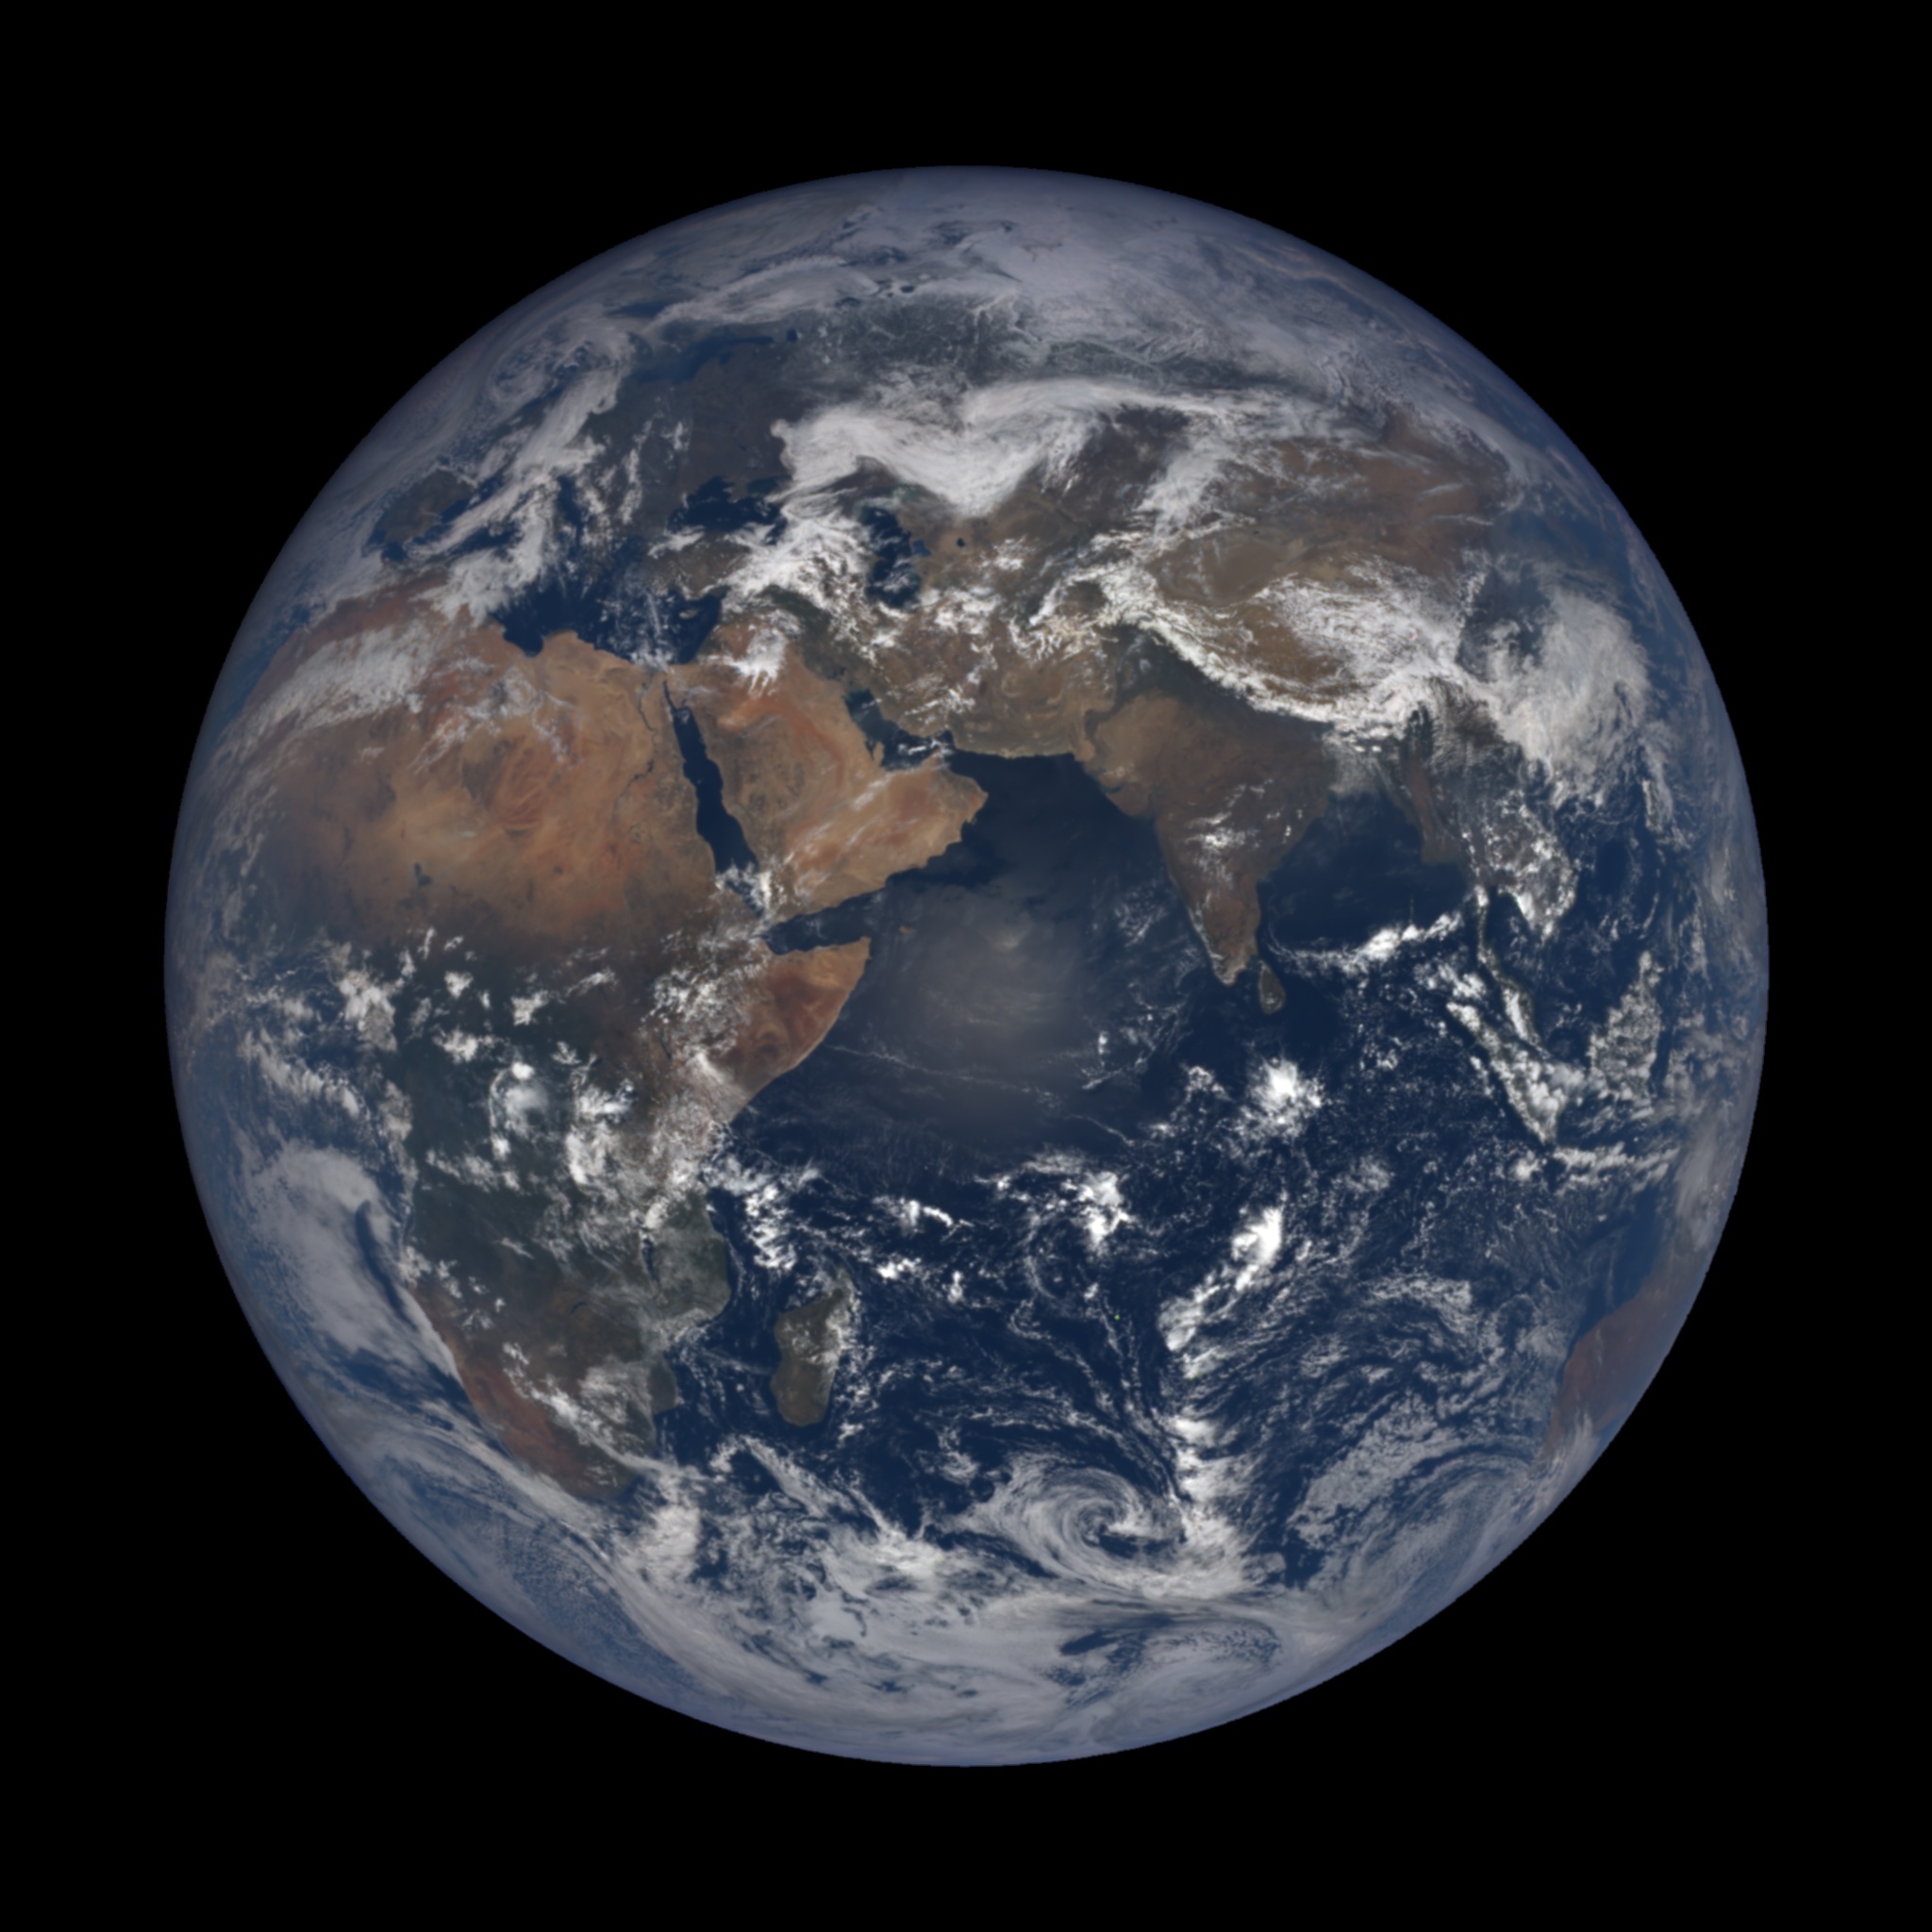
\includegraphics[width=5cm]{images/dscovrepic/epic1}
%	\end{center}
%	
%	\vfill
%\end{frame}
%}


\begin{frame}
	\frametitle{System Earth}
	
	\begin{columns}

	\column{.5\textwidth}
	
	{
%		The Earth is a complex system.
%		Only some components is observable by 
%		\begin{itemize}
%			\item satellite-based or
%			\item in-situ observations
%		\end{itemize}
%		
		
%	\begin{equation*}\V{y} = f({\M{X}})\end{equation*}
%	partially observe the complex system Earth
	\textbf{Partially measuring} System Earth
	{\Huge
		\begin{equation*}
			\M{X} = \sat\left({\earth}\right)
		\end{equation*}
	}

	\vspace{1em}
	\textbf{knowledge extraction} through pattern recognition and machine learning
	
	{\Huge\begin{equation*}\V{?} = f({\M{X}})\end{equation*}}
	}

	\column{.5\textwidth}
	
	\begin{tikzpicture}[xscale=3, yscale=2]
		\node(earth) at (0,0) {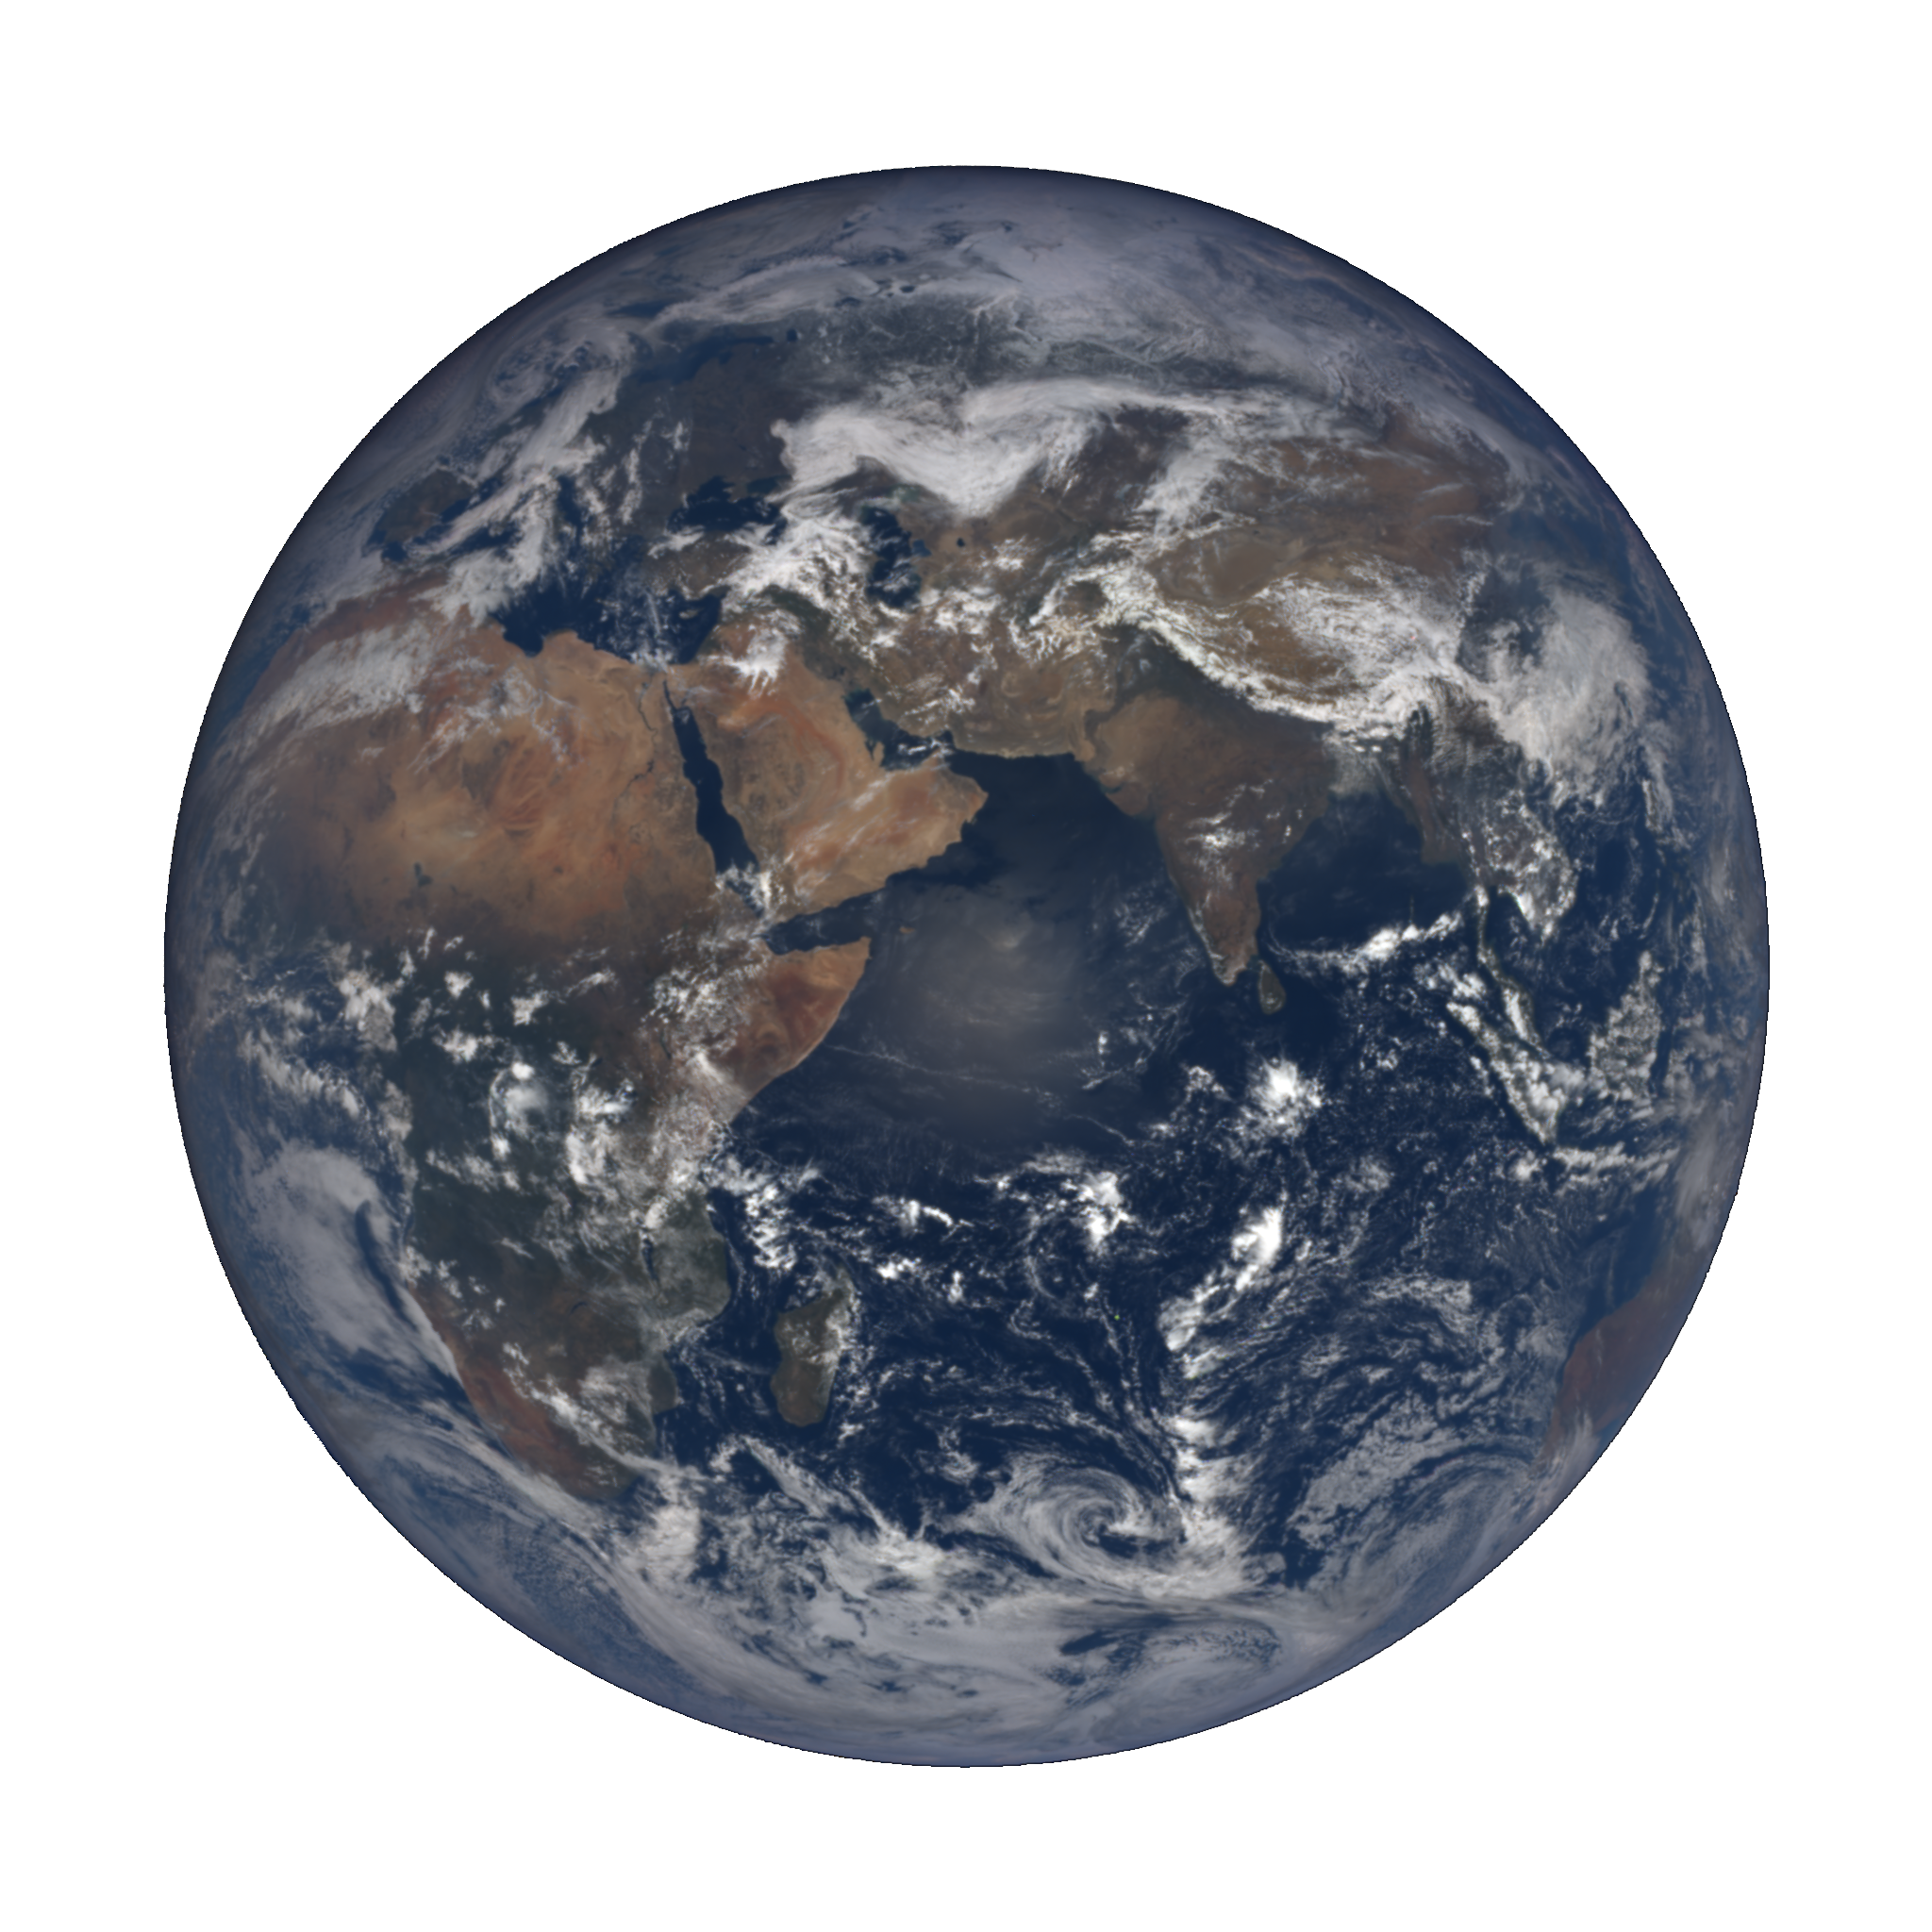
\includegraphics[width=7cm]{images/dscovrepic/epicw1}};	

	\end{tikzpicture}
	
	
	\end{columns}

%	\includegraphics[width=5cm]{images/Earth_gravity}
%	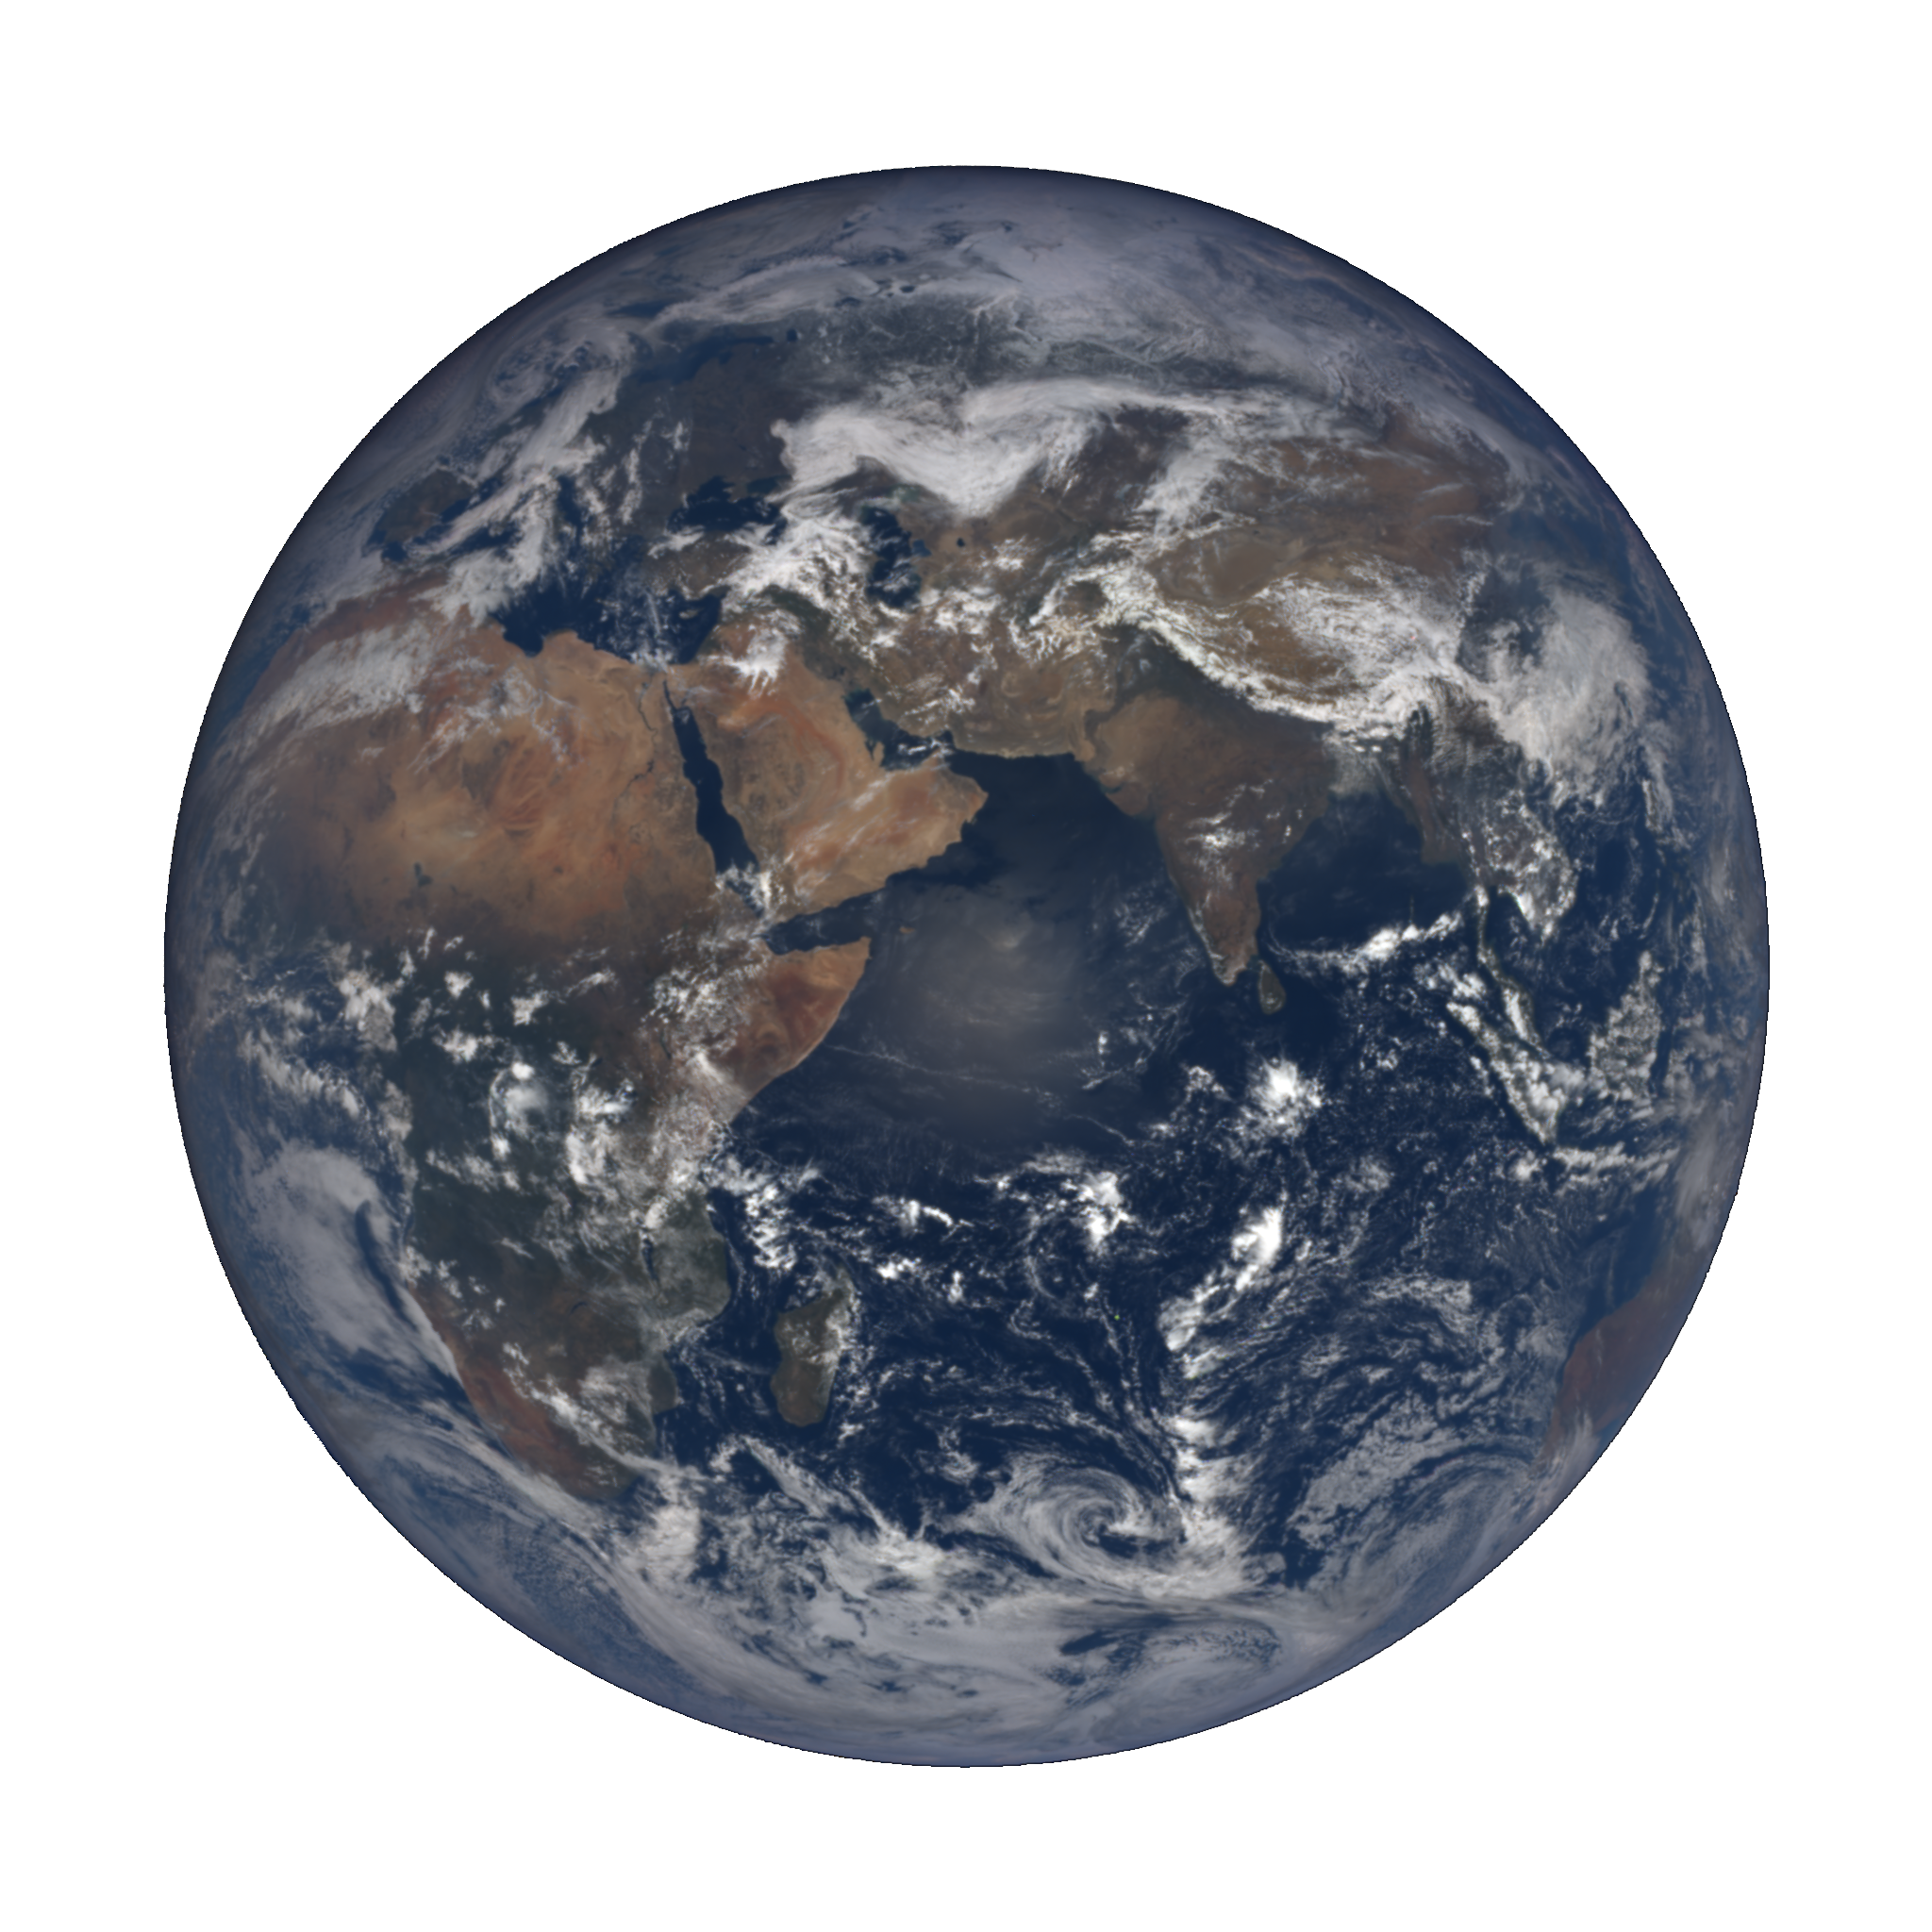
\includegraphics[width=5cm]{images/dscovrepic/epicw1}
%	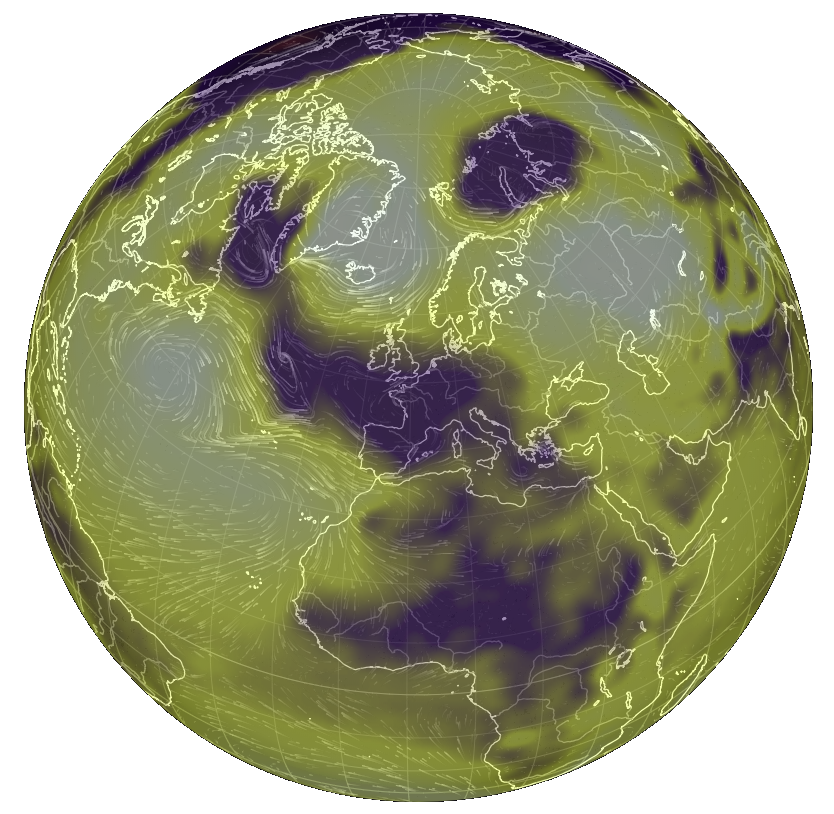
\includegraphics[width=5cm]{images/earthnullschool/sealevelpressure}
%	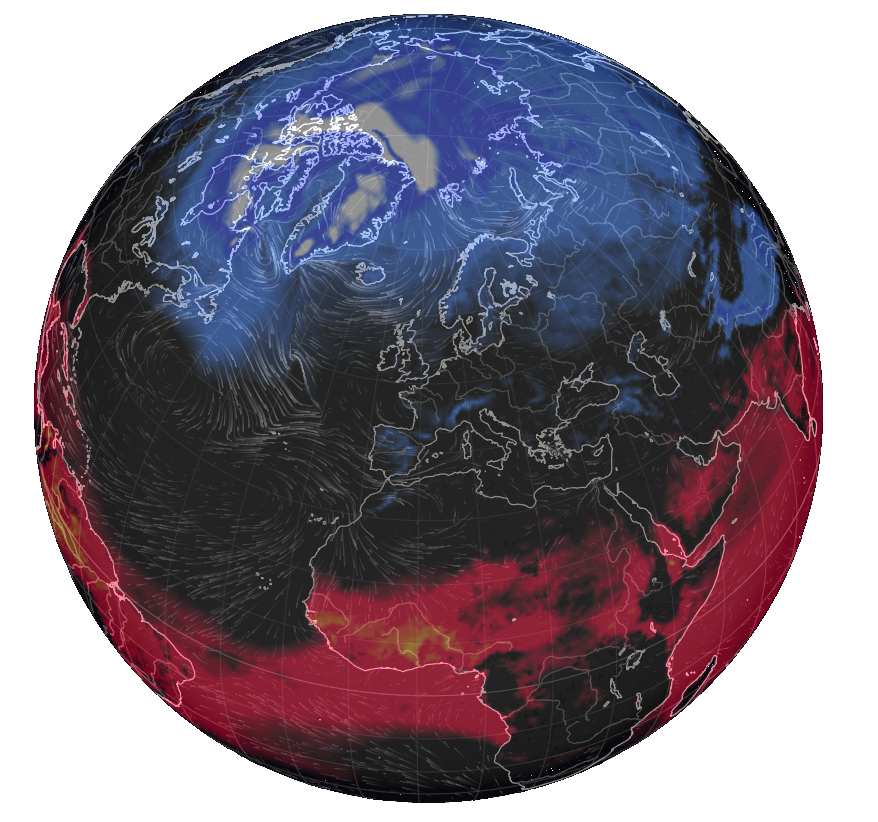
\includegraphics[width=5cm]{images/earthnullschool/misery_index}
%	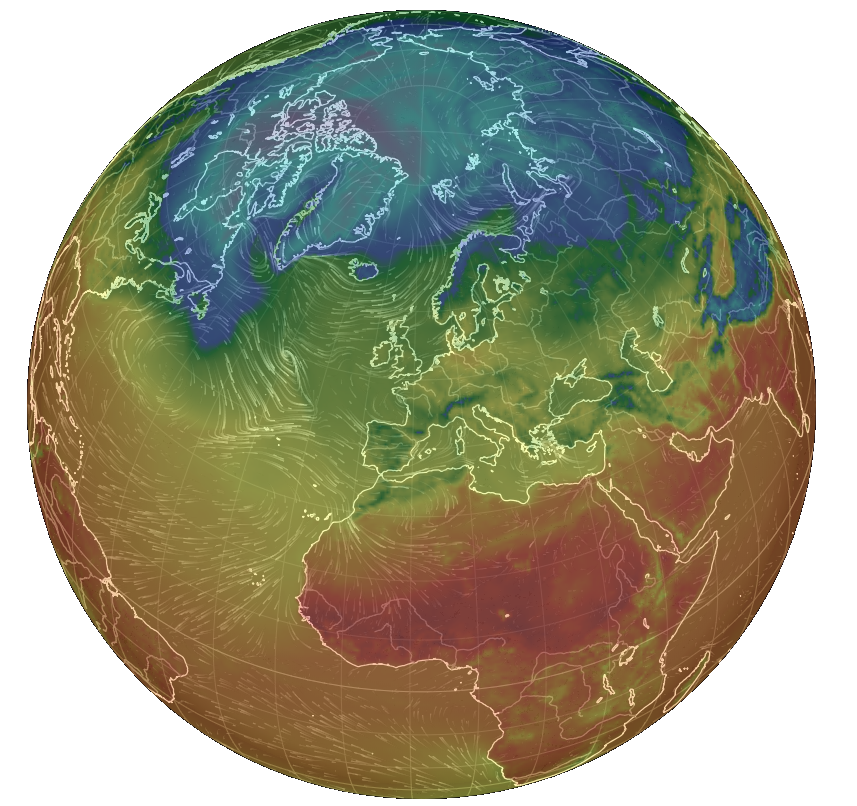
\includegraphics[width=5cm]{images/earthnullschool/temp}
%	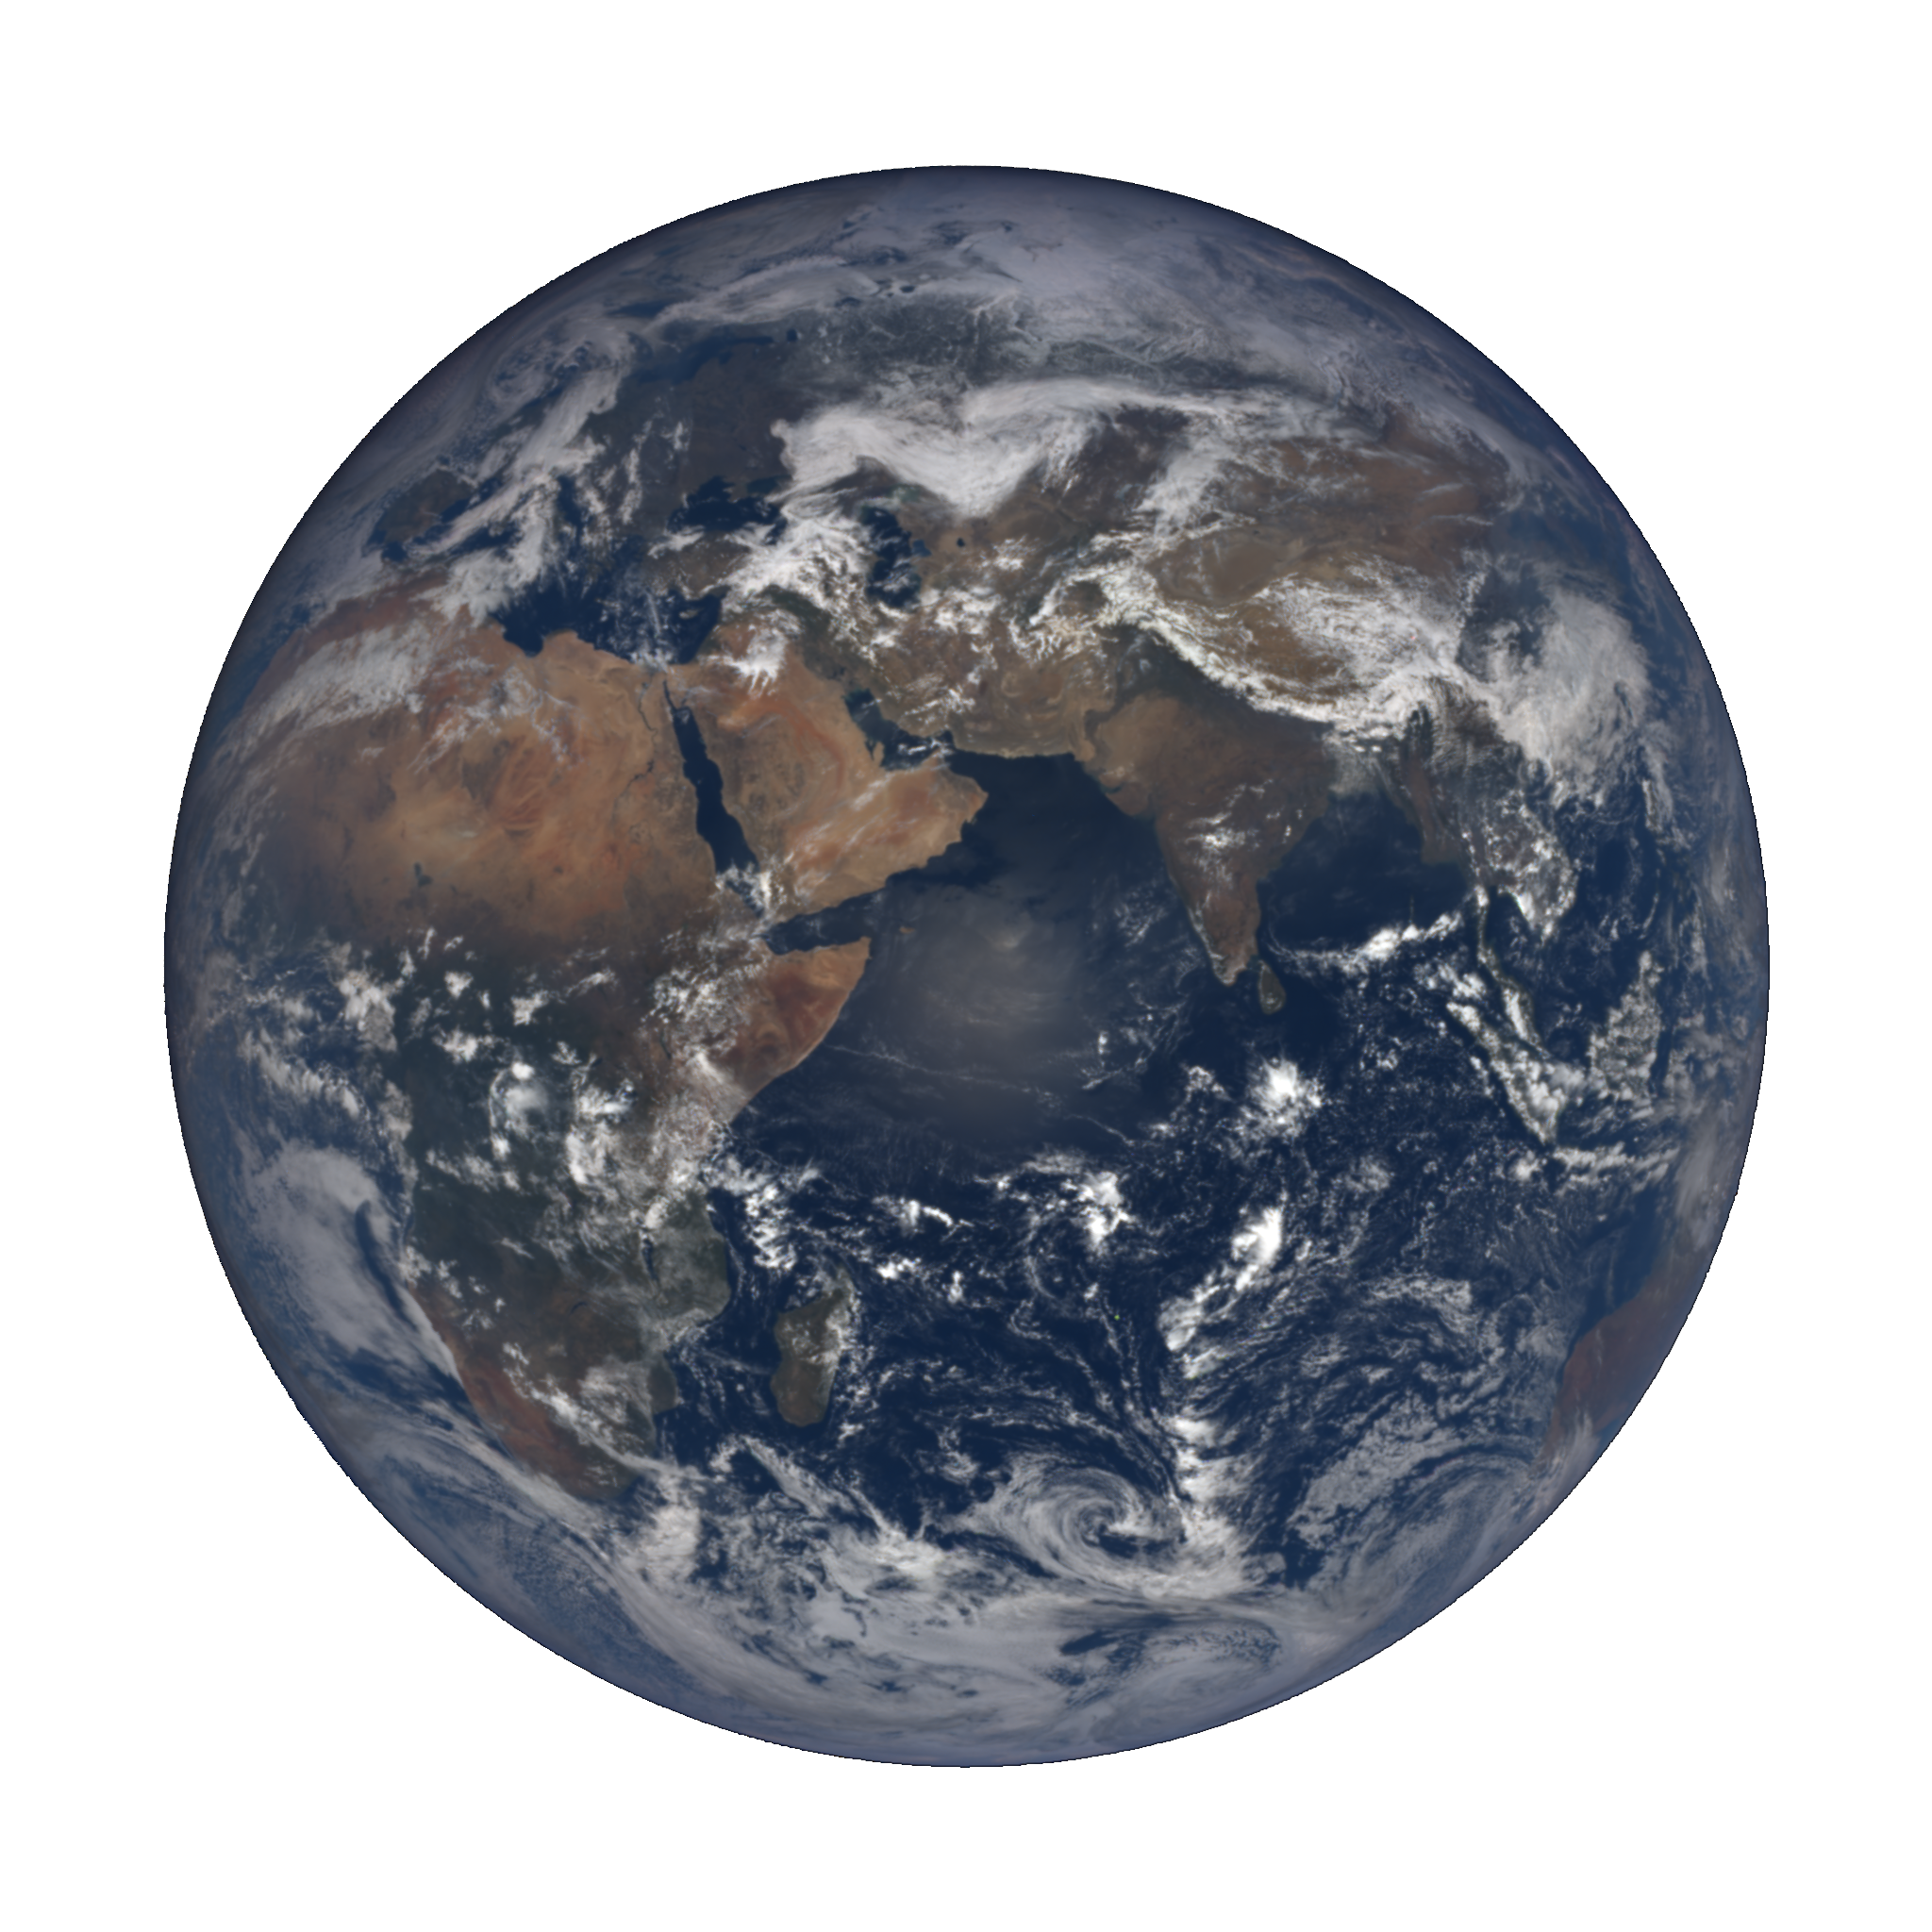
\includegraphics[width=5cm]{images/dscovrepic/epicw1}
	\end{frame}
%
%\begin{frame}
%	\frametitle{Measurements}
%	
%	\begin{columns}
%	
%	\columnwidth{.5\textwidth}
%	In-Situ Measurements
%	\begin{itemize}
%		\item Seismographs
%		\item Flux-Towers
%		\item Weather Stations
%		\item GNSS ground station
%		\item ...
%	\end{itemize}
%
%	Satellite-based Sensors
%	\begin{itemize}
%		\item Gravimetry
%		\item GNSS Science
%		\item Atmospheric Sciences
%		\item Radar (Active Sensors)
%		\item Optical Satellite Sensors
%	\end{itemize}
%
%	\columnwidth{.5\textwidth}
%
%	\begin{tikzpicture}
%		content...
%	\end{tikzpicture}
%
%	\end{columns}
%
%\end{frame}

%
\begin{frame}
\frametitle{Passive Optical Sensors}
\begin{columns}
	\column{.5\textwidth}
	
	
	\begin{itemize}[itemsep=.5em]
		\item<1-> Sensor measures \textbf{Digital Numbers} $\text{DN}(\lambda)$ for each band wavelength $\lambda$. 
		\item<2-> \textbf{Digital Numbers} are normalized to \textbf{Radiance} 
		$L(\lambda), \left[\frac{W}{\text{sr}m^1}\right]$ by gain and offset calibration.
		\item<4-> Radiance is normalized to \textbf{top-of-atmosphere reflectance} $\rho(\lambda)$
		\item<4-> \textbf{Bottom-of-atmosphere reflectances} are reconstructed using a functional model of the atmosphere.
	\end{itemize}
	
%	Radiance $R_\lambda$ from measured Digital Numbers via calibrated gain $\alpha$ and offset $\beta$
%	\begin{equation*}
%		L_\lambda = \alpha \text{DN}_\lambda + \beta, \left[\frac{W}{\text{sr}m^1}\right]
%	\end{equation*}
%	
%	top-of-atmosphere reflectance $\rho_\lambda$ as normalized Radiance $R_\lambda$ with solar 
%	\begin{equation*}
%	\rho_\lambda = \frac{L_\lambda}{\cos(\varphi_\text{sun})}
%	\frac{
%		\pi d^2
%	}
%	{
%		E_\text{sun}(\lambda)
%	}
%	\end{equation*}
%	
%	\vspace{1em}
%	
%	\begin{itemize}
%		\item measured radiance $L(\lambda)$
%		\item solar irradiance $E_\text{sun}(\lambda)$
%		\item solar zenith angle $\varphi_\text{sun}$
%		\item squared Earth-Sun distance $d$ in AU
%	\end{itemize}

	
	\column{.5\textwidth}
	
	
	\begin{tikzpicture}
	
	
	%	\draw [black,dotted, fill=tumbluelight,domain=110:70] plot ({13*cos(\x)}, {13*sin(\x)-12.8});
	\draw [fill=tumivory,domain=110:70] plot ({10*cos(\x)}, {10*sin(\x)-10});
%	\draw [fill=tumbluelight,domain=110:70] plot ({12*cos(\x)}f, {12*sin(\x)-10});
	
	
	\node(sun) at (-2,2) {
\includegraphics[width=10mm]{images/icons/sun}};
	\node[rotate=130,anchor=center](sat) at (2,2) {
\includegraphics[width=10mm]{images/icons/sat2}};
	
	\node(px) at ({10*cos(90)}, {10*sin(90)-10.1}){
		\begin{tikzpicture}[xscale=.5,yscale=.25]
		\draw[fill=tumbluelight] (0,0) -- (1,0) -- (2,1) -- (1,1) -- (0,0);
		\end{tikzpicture}
		%
\includegraphics[width=5mm]{images/icons/house}
	};
	
	\draw[-stealth] (sun) -- node[midway,sloped]{\wave} (px);
	\draw[-stealth] (px) -- node[midway,sloped]{\wave} (sat);
	
	\visible<3->{\draw[-stealth] (sun) -- node[midway,sloped]{\wave} (sat);
	\draw[draw=tumgray] (px) -- node[at end,left]{$\varphi_\text{sun}$} ++(0,1.4); 
	\draw [draw=tumgray, domain=130:90] plot ({1*cos(\x)}, {1*sin(\x)});
	}
	
	\node[above=.5em of sun]{$E_\text{sun}(\lambda)$};
	\visible<1>{\node[above=4em of sat]{$DN(\lambda)$};}
	\visible<2>{\node[above=4em of sat]{$L(\lambda)$};}
	\visible<3>{\node[above=4em of sat]{$\rho_\text{toa}(\lambda)$};}
	\visible<4>{\node[above=4em of sat]{$\rho_\text{boa}(\lambda)$};}

	%		\draw[red] (0,0) sin (1,2);
	
	\end{tikzpicture}
	
\end{columns}

\end{frame}

\newcommand{\rastergrid}{
	\begin{tikzpicture}
	% each layer
	\begin{scope}[scale=2]
	
	% raster size
	\def\d{0.7}		
	
	% distance layer
	\def\s{\d*5}
	
	\foreach \i in {1,...,6}
	{		
		\begin{scope}[
		yshift=\s*\i,every node/.append style={
			yslant=0.5,xslant=-1},yslant=0.5,xslant=-1
		]
		%\draw[step=3.33mm] (0,0) grid (1,1);
		%\fill[black,fill opacity=.9] (0.333,0.333) rectangle (0.333,0.333);    	    	  
		
		\foreach \row in {0,...,2}{
			\foreach \col in {0,...,2}{
				\draw[tumblack, fill=tumblue!\pdfuniformdeviate 40,fill opacity=1,rounded corners=1] (\col*\d/3,\row*\d/3) rectangle (\col*\d/3+\d/3, \row*\d/3+\d/3);
				%                 \draw[black, fill=black!\pdfuniformdeviate 40,fill opacity=1,rounded corners=1] (\col*\d/3,\row*\d/3) rectangle (\col*\d/3+\d/3, \row*\d/3+\d/3);
			}
		}
		
		%\draw[step=3.33mm] (0,0) grid (1,1);
		%\fill[white,fill opacity=.9] (0,0) rectangle (1,1);
		\end{scope}
	}
	\end{scope}
	\end{tikzpicture}
}


%\begin{frame}
%\frametitle{Spectral Band}
%\end{frame}


\newcommand{\myvec}[1]{\ensuremath{\begin{pmatrix}#1\end{pmatrix}}}
\begin{frame}
\frametitle{Spatial and Temporal Discretization}

\begin{columns}
	\column{.5\textwidth}
	
	{
		\begin{equation*}
		\M{X} = \myvec{\rho_{\lambda_1} \\ \rho_{\lambda_2} \\ \dots \\ \rho_{\lambda_n}}
		\end{equation*}
	}
	
	
	
	Spectral reflectance of \textbf{spectral bands} disctretized on a \textbf{spatial grid}. Each grid cell is georeferenced by its Longitude $\Lambda$ and Latitude $\Phi$.
	Acquisitions in regular \textbf{temporal intervals}.
	
	\column{.5\textwidth}
	
	
	
	\begin{tikzpicture}
	
	%	\node(a){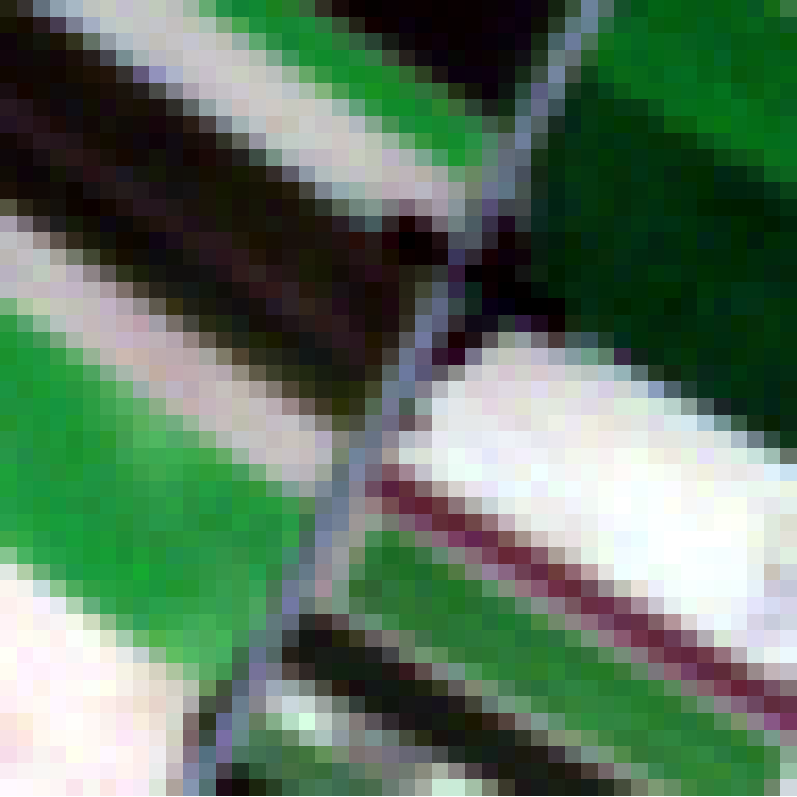
\includegraphics[width=3cm]{images/s2grid/1}};
	
	%	\draw[step=1cm,gray,very thin] (-2,-2) grid (6,6);
	
	
	\draw [fill=tumivory,domain=110:70] plot ({11*cos(\x)}, {11*sin(\x)-8.5});
	
	\begin{scope}[scale=1]
	
	% raster size
	\def\d{1}		
	
	% distance layer
	\def\s{\d*50}
	
	\node at (-1.7,2.4){$t_{i-1}$};
	\node at (-1.7,4.2){$t_i$};
	\node at (-1.7,6){$t_{i-1}$};
	
	\node at (1,1.9){$\Lambda$};
	\node at (-1,1.9){$\Phi$};
	
	%		\draw[step=1.0,black,thin] (-2,0) grid (2,5);
	
	
	\foreach \i in {1,...,3}
	{		
		
		\begin{scope}[
		yshift=\s*\i,every node/.append style={
			yslant=0.5,xslant=-1},yslant=0.5,xslant=-1,scale=0.35
		]
		%\draw[step=3.33mm] (0,0) grid (1,1);
		%\fill[black,fill opacity=.9] (0.333,0.333) rectangle (0.333,0.333);    	    	  
		
		
		
		\foreach \row in {0,...,3}{
			\foreach \col in {0,...,3}{
				\draw[tumblack, fill=tumblue!\pdfuniformdeviate 40,fill opacity=1,rounded corners=1] (\col,\row) rectangle (\col+1, \row+1);
				
				\node[font=\tiny, text=tumblue] at (\col + 0.5,\row + 0.5) {$\V{x}$};
				
				%                 \draw[black, fill=black!\pdfuniformdeviate 40,fill opacity=1,rounded corners=1] (\col*\d/3,\row*\d/3) rectangle (\col*\d/3+\d/3, \row*\d/3+\d/3);
			}
		}
		
		%\draw[step=3.33mm] (0,0) grid (1,1);
		%\fill[white,fill opacity=.9] (0,0) rectangle (1,1);
		\end{scope}
	}
	\end{scope}
	
	
	
	\end{tikzpicture}
	
\end{columns}


%	\begin{equation*}
%		x_{geo} = \begin{pmatrix} \Lambda \\ \Phi\end{pmatrix} + x_{image} \begin{pmatrix}px_w & 0 \\ 0 & px_h\end{pmatrix}
%	\end{equation*}

\end{frame}


\begin{frame}

\vfill
\Huge\color{black}
\begin{center}
	\begin{columns}
		\column{\textwidth}
		\vspace{7em}
		
		\textbf{Hands-on:}
		\hfill 
		Optical Earth Observation
		%			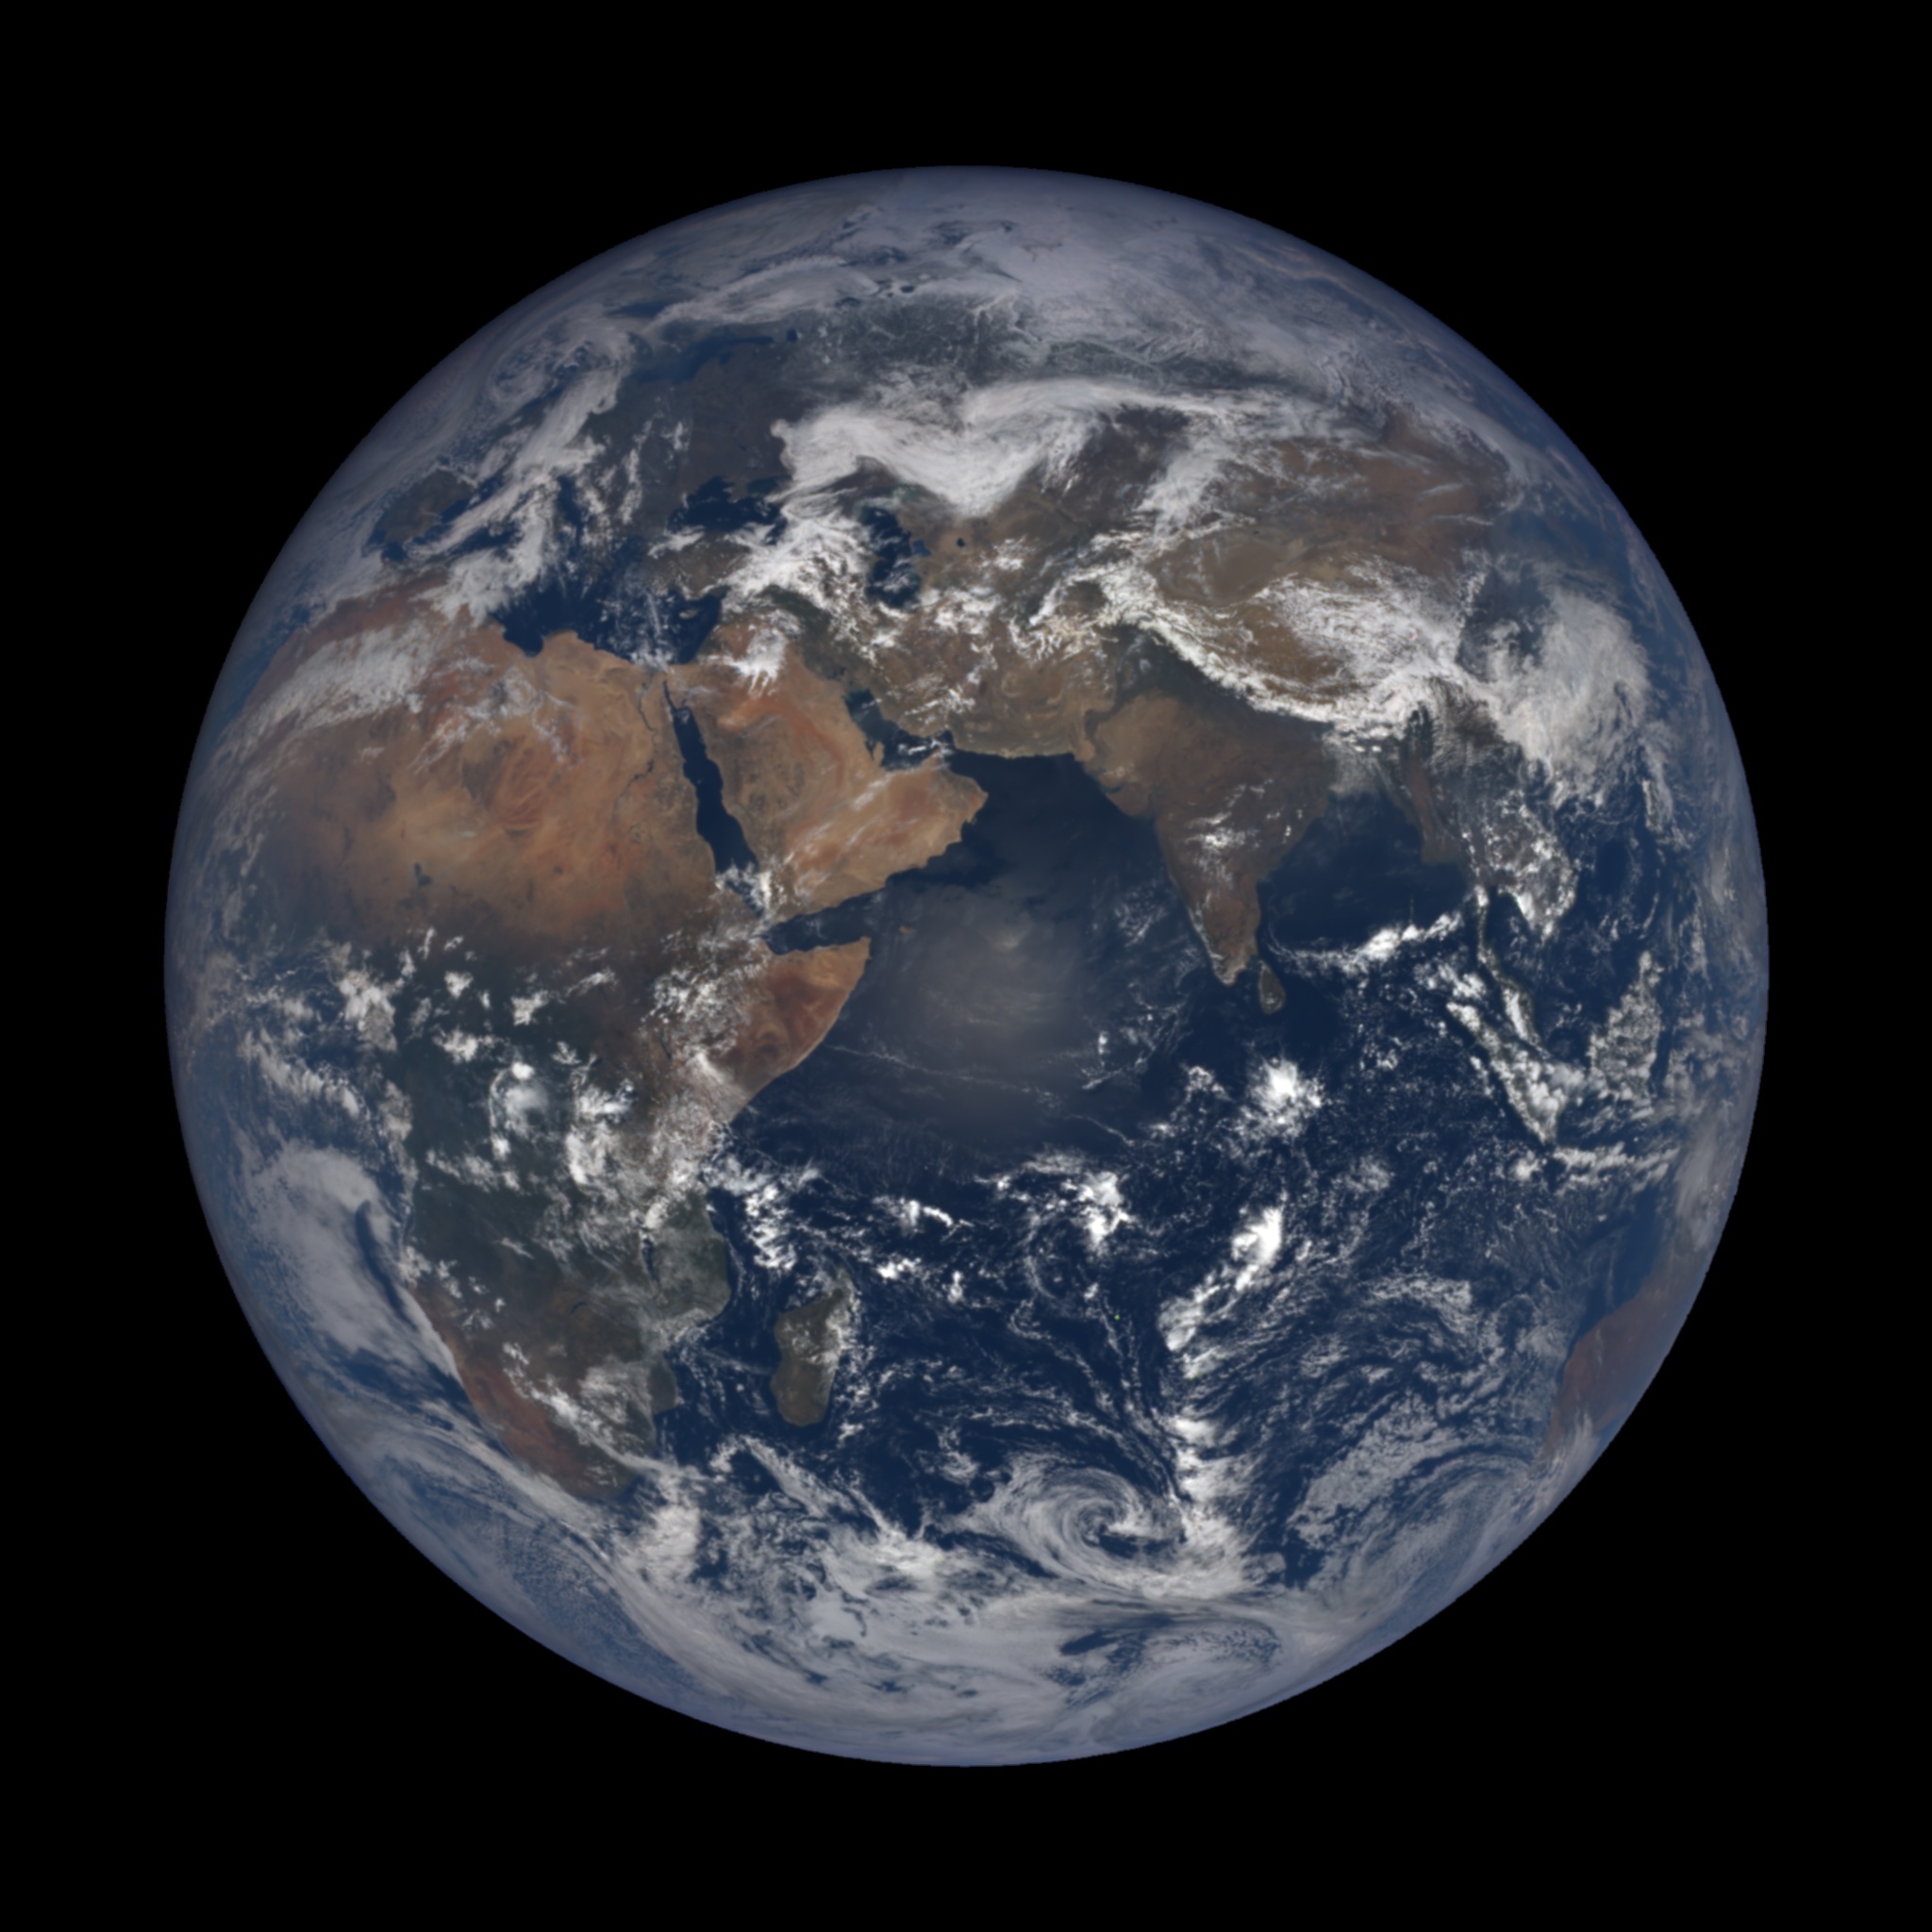
\includegraphics[width=5cm]{images/dscovrepic/epic1}
		%
\includegraphics[width=7cm]{images/fdl}
	\end{columns}
\end{center}

\vfill

\end{frame}


%
%\end{document}




{	
%	\setbeamercolor*{Title bar}           {bg=tumblack,fg=tumblue}
%	\setbeamercolor*{Location bar}        {bg=tumblack,fg=tumblue}
%	\setbeamercolor*{frametitle}          {parent=Title bar}
%	\setbeamercolor*{normal text}         {bg=tumblack,fg=tumwhite}
%	
	
\tikzstyle{dist} = [font=\tiny]
	
\begin{frame}
  \frametitle{Weather Satellites}
  \framesubtitle{At the Langrange 1 Point}
  
  
  
  
  \begin{columns}
  	\column{.3\textwidth}
  	
  	\hspace{2em}\textbf{dscovr:epic}
  	\begin{itemize}
  		\item 8 km spatial resolution
  		\item image every 20s
  		\item 10 spectral channels
  	\end{itemize}
  	
  	\column{.3\textwidth}
  	\hspace{2em}
  	\begin{tikzpicture}
  	
  	
  	
  	\visible<1>{\node[rotate=-20, anchor=center](earth) at (0,0) {
\includegraphics[width=5mm]{images/icons/earth}};}
  	\visible<2>{\node[rotate=0, anchor=center](earth) at (0,0) {
\includegraphics[width=5mm]{images/icons/earth}};}
  	\visible<3>{\node[rotate=20, anchor=center](earth) at (0,0) {
\includegraphics[width=5mm]{images/icons/earth}};}
  	\visible<4>{\node[rotate=40, anchor=center](earth) at (0,0) {
\includegraphics[width=5mm]{images/icons/earth}};}
  	
  	\only<4>{\node at (-.2,-1) {
\includegraphics[width=3mm]{images/icons/moon}};};
  	
  	\node[anchor=center](sat) at (0,-2) {
\includegraphics[width=5mm]{images/icons/sat2}};
  	\node at (0,-4) {
\includegraphics[width=5mm]{images/icons/sun}};
  	
  	\draw[dist] (earth) -- node[midway,below,sloped]{1.5 Mio km} (sat);
  	
  	\node[left=1em of sat, text=white]{$L_1$};
%  	\draw [red,thick,domain=230:315] plot ({2*cos(\x)}, {2*sin(\x)});
  	\end{tikzpicture}
  	
  	\column{.7\textwidth}
  	
  	\only<1>{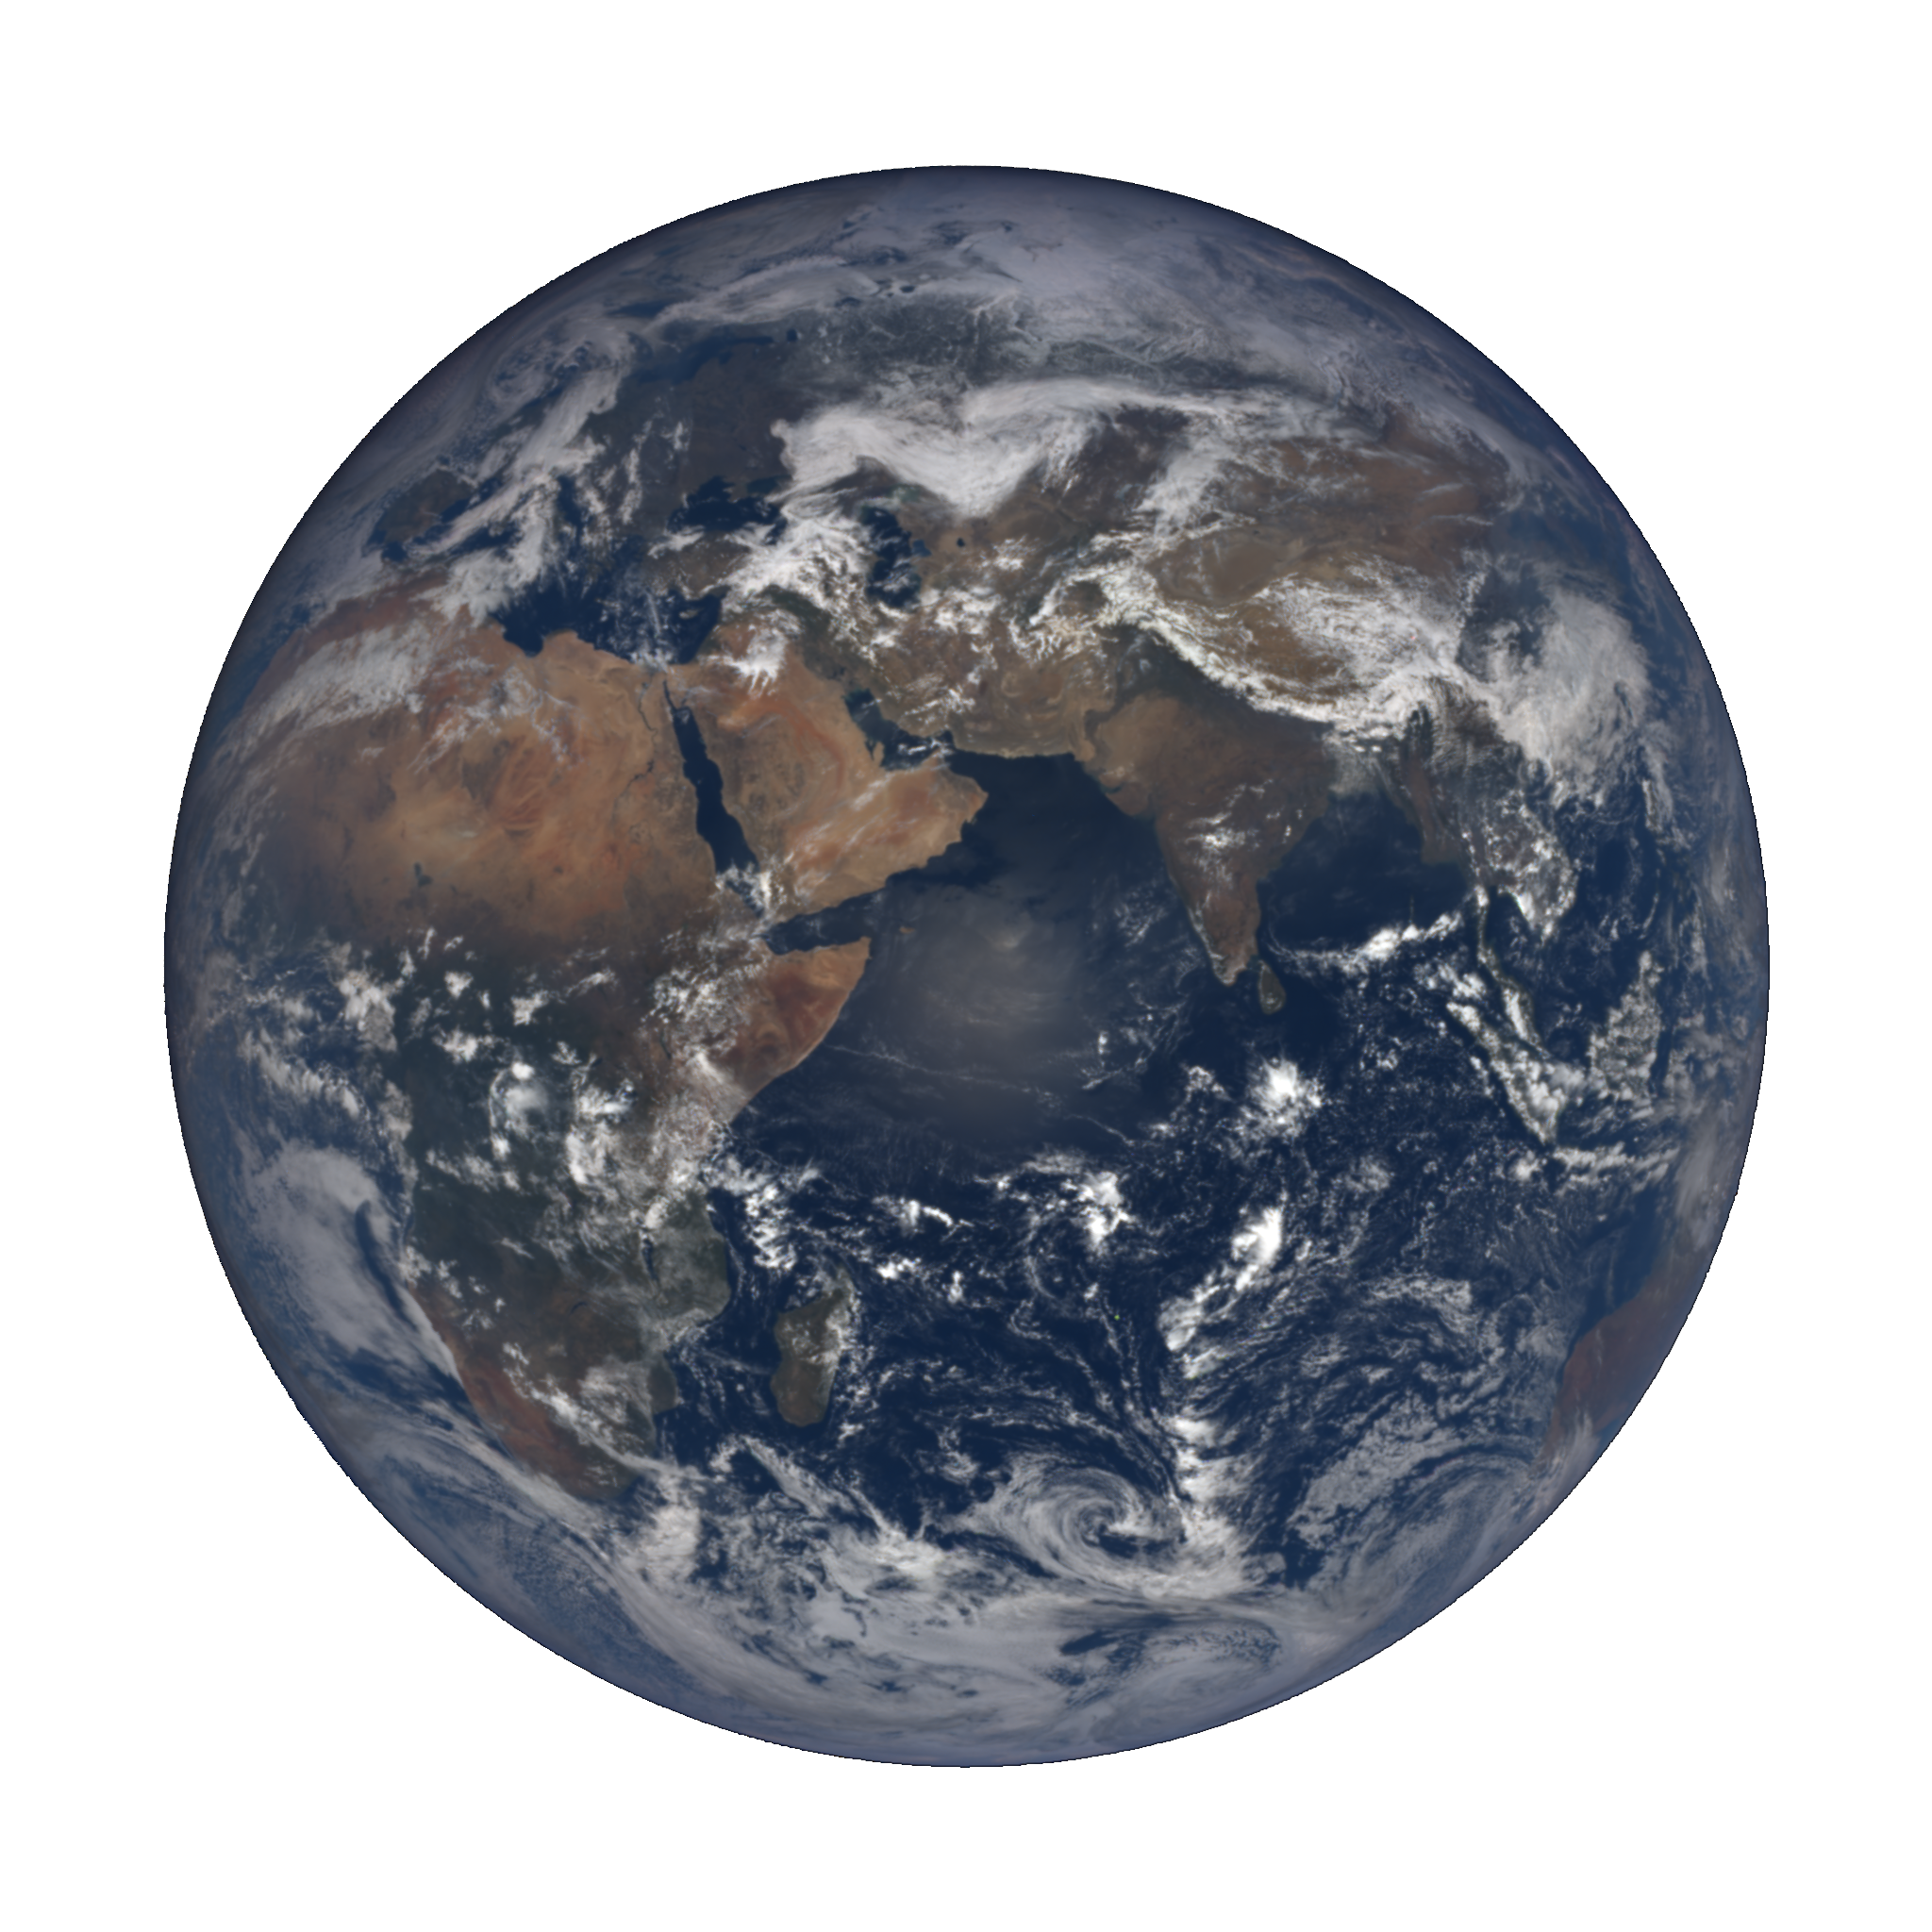
\includegraphics[width=6cm]{images/dscovrepic/epicw1}}
  	\only<2>{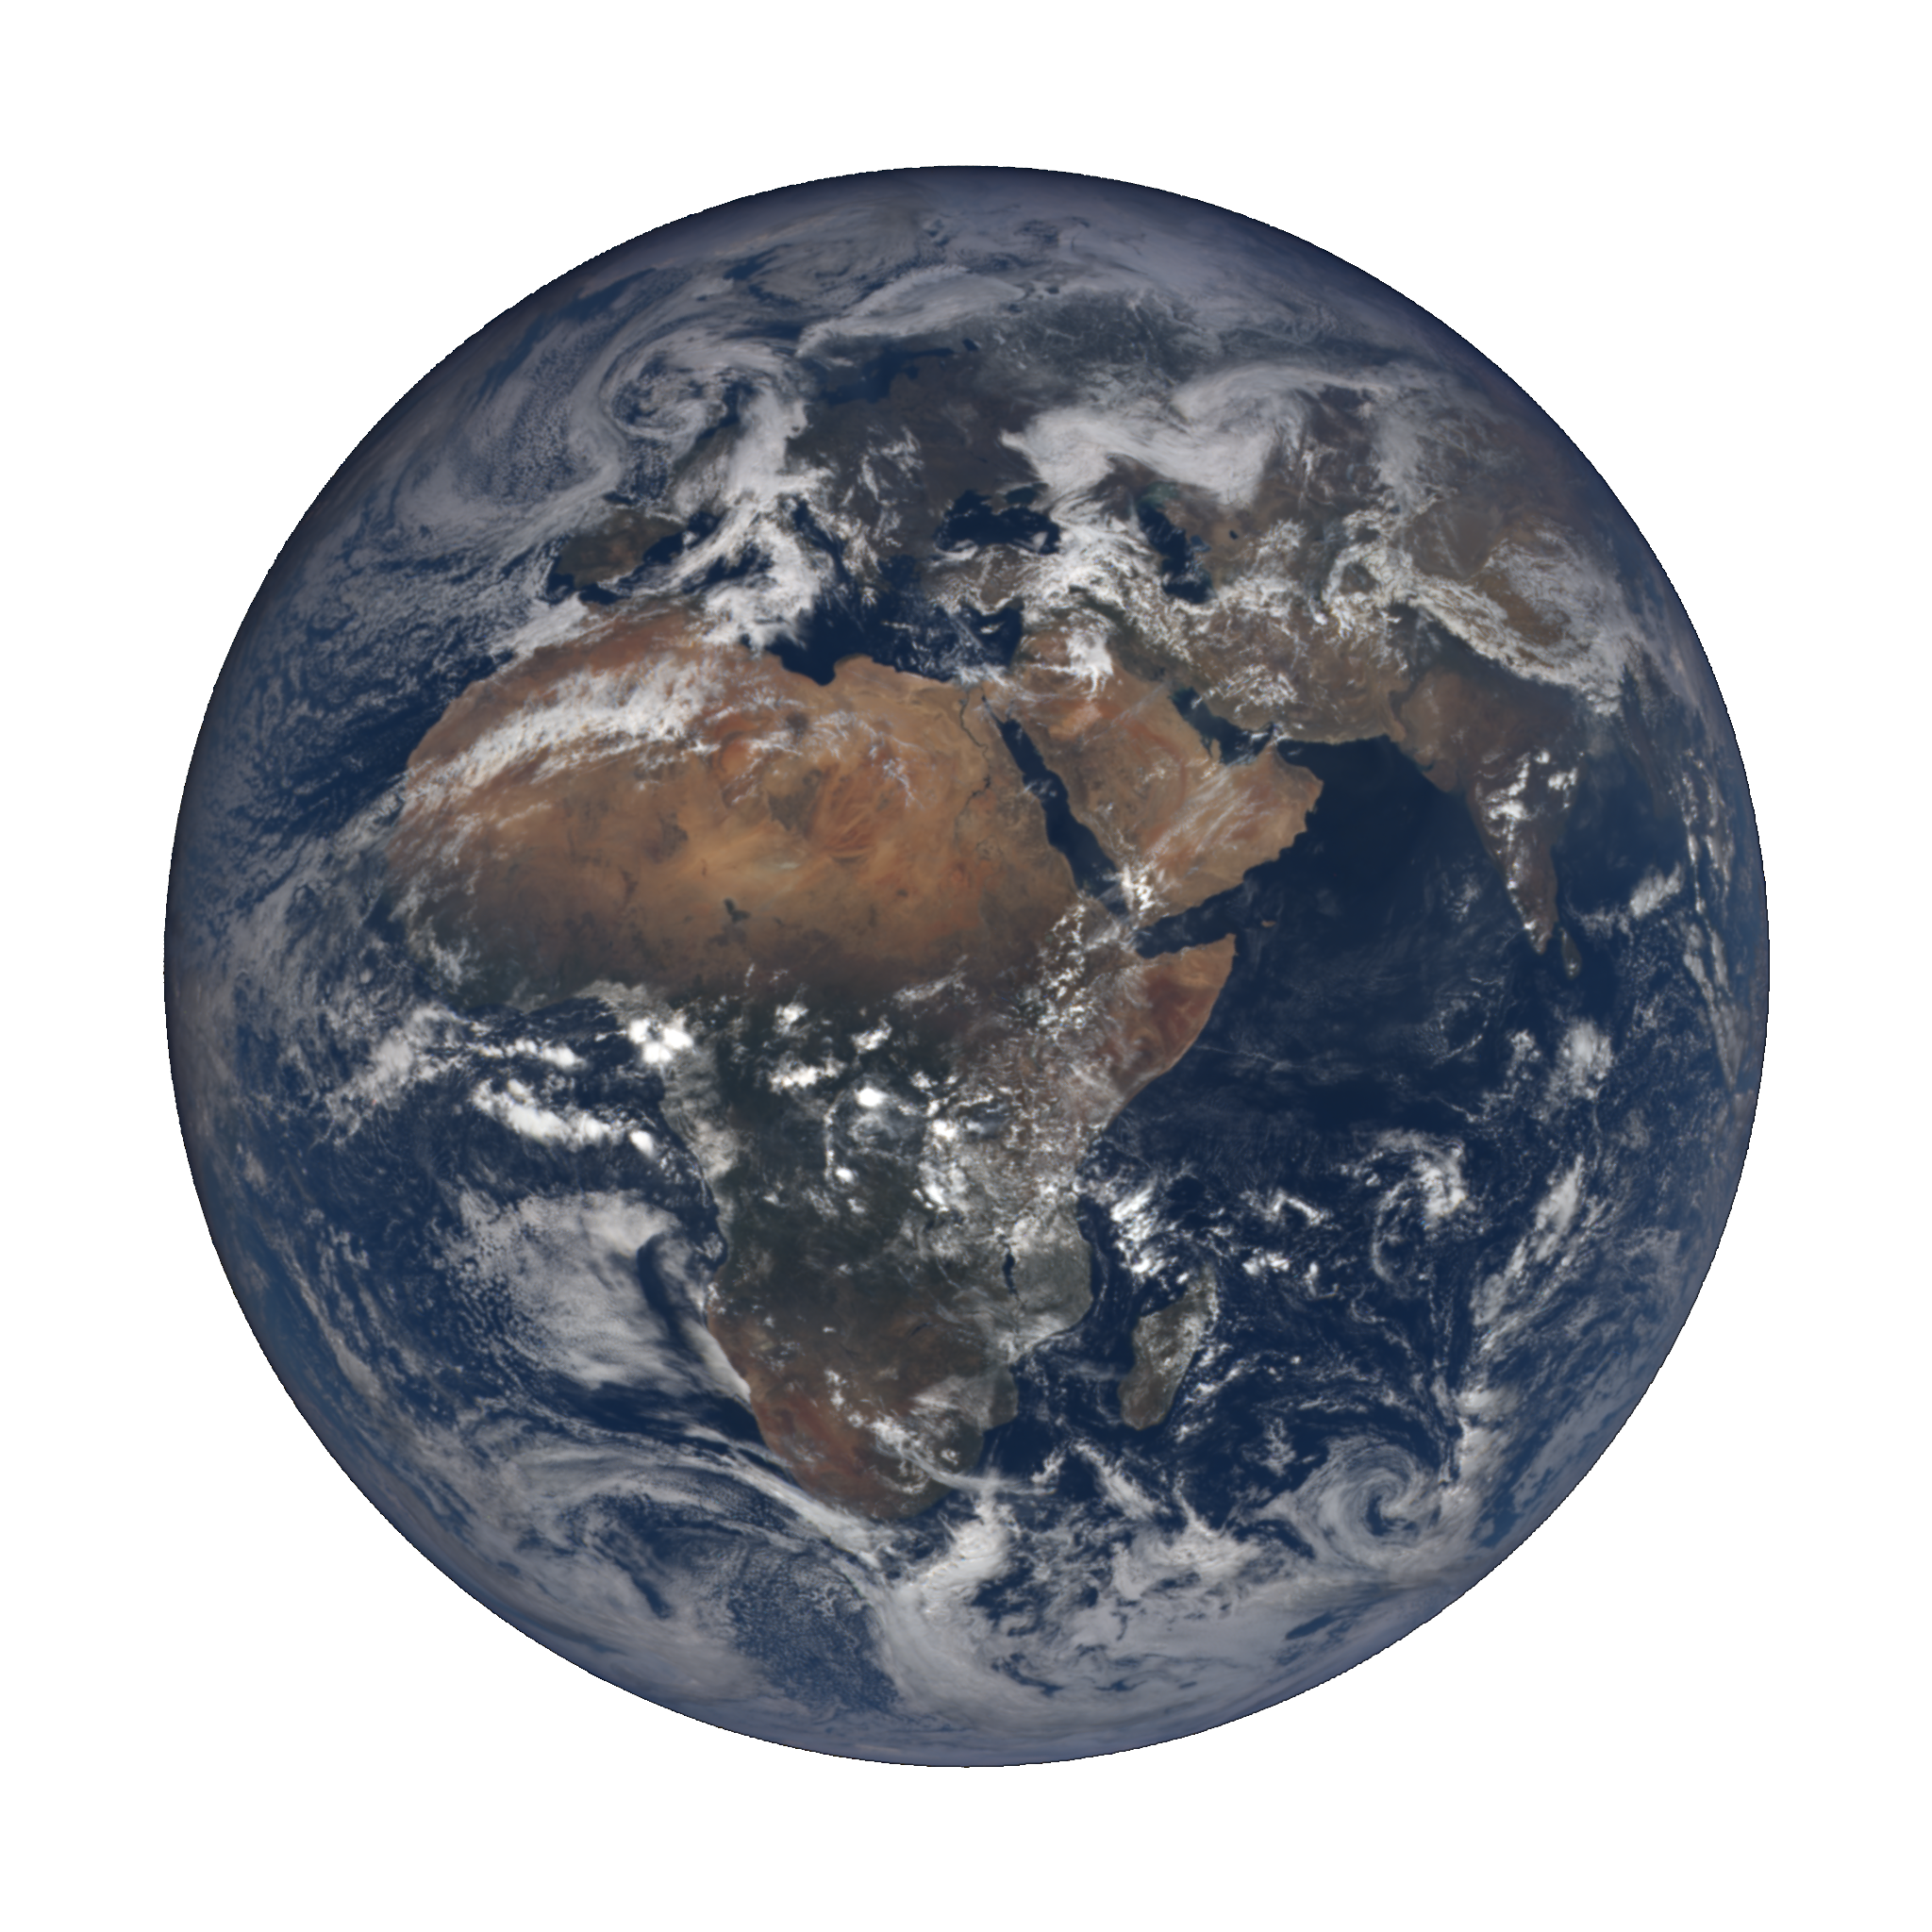
\includegraphics[width=6cm]{images/dscovrepic/epicw2}}
  	\only<3>{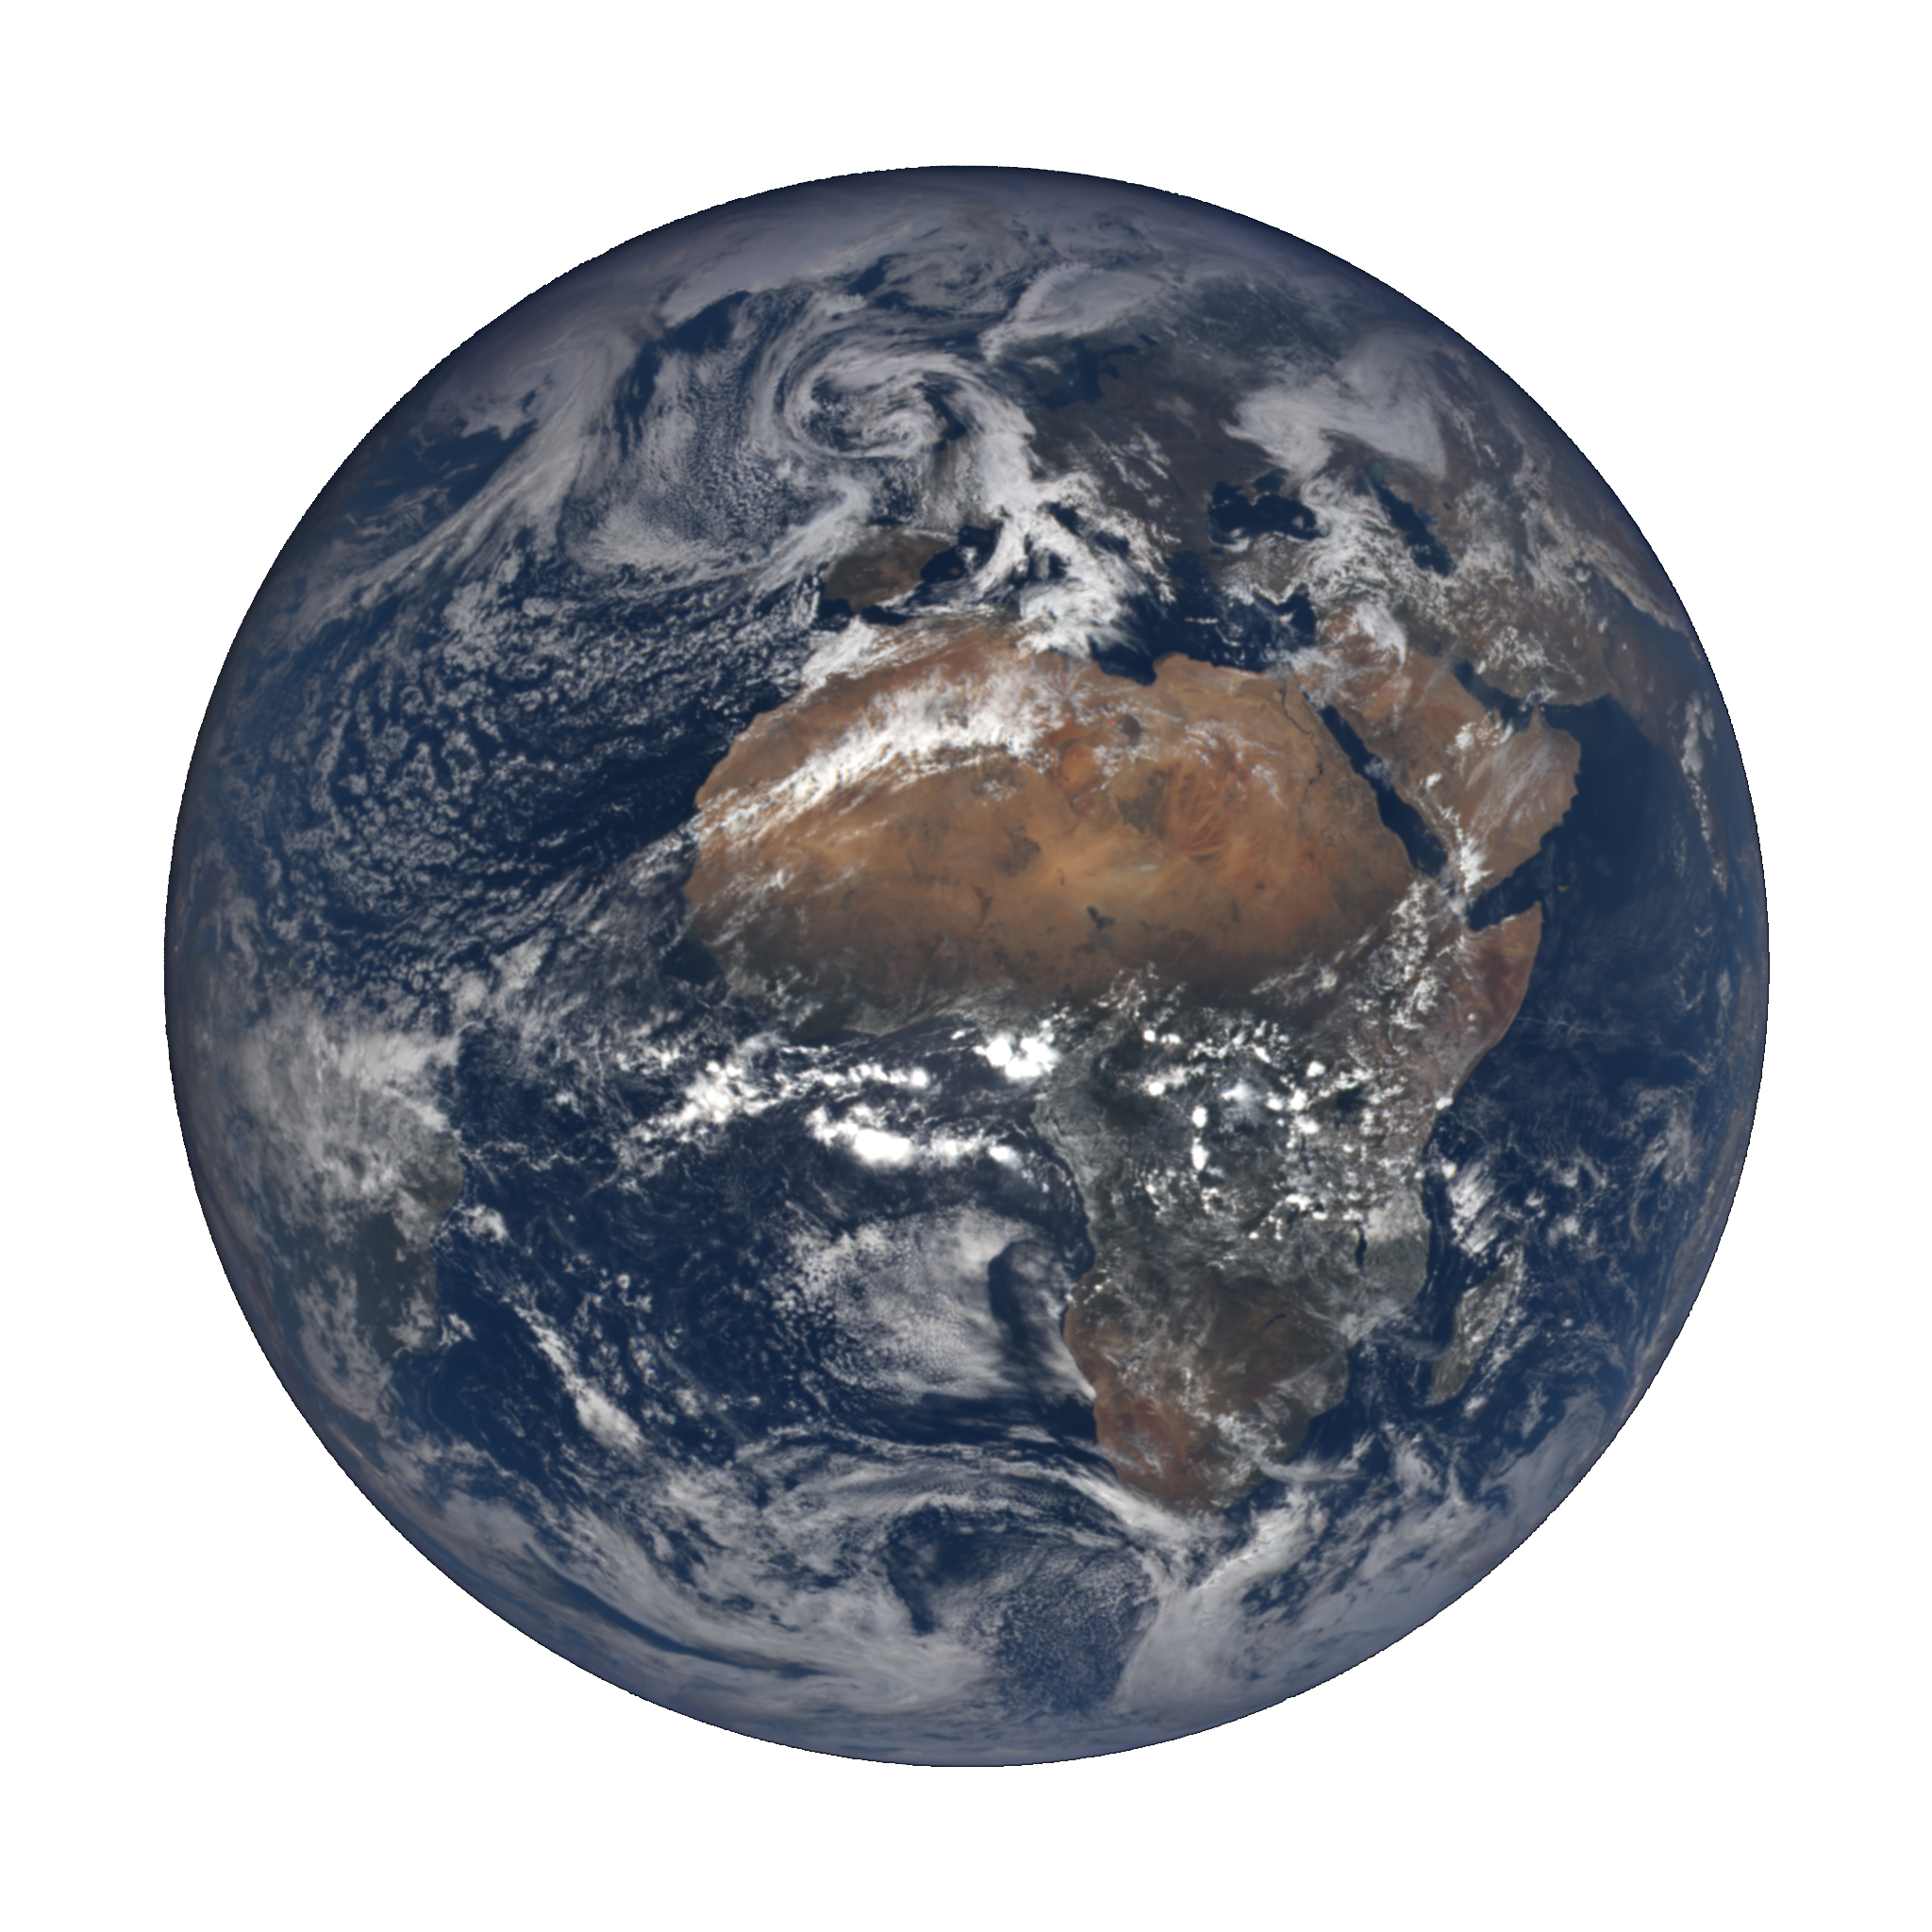
\includegraphics[width=6cm]{images/dscovrepic/epicw3}}
  	\only<4>{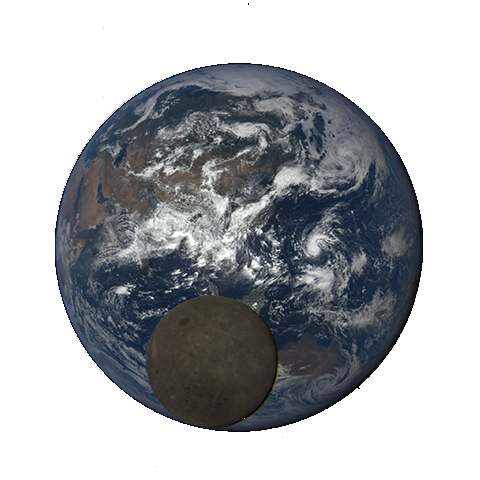
\includegraphics[width=6cm]{images/dscovrepic/epicwl2}}

\end{columns}

\url{twitter.com/dscovr_epic}
\url{epic.gsfc.nasa.gov}

\hfill
\vfill
\scriptsize Icons from \url{https://www.flaticon.com}
 \end{frame}

\begin{frame}
\frametitle{Weather Satellites}
\framesubtitle{At geostationary orbit}


\begin{columns}
	\column{.3\textwidth}
	
	\hspace{2em}\textbf{MeteoSAT, GOES}
	\begin{itemize}
		\item 2.5 - 5km km spatial resolution
		\item image every 15 minutes
		\item 12 spectral 0channels
	\end{itemize}
	
	
	\column{.3\textwidth}
%	\hspace{2em}
	\begin{tikzpicture}
	
	
	\draw [tumgraylight,dotted,domain=230:315] plot ({2*cos(\x)}, {2*sin(\x)});
	
	\visible<1>{
	\node[rotate=-20, anchor=center](earth) at (0,0) {
\includegraphics[width=5mm]{images/icons/earth}};
	\node[anchor=center, rotate around={-20:(0,2)}](sat) at (0,-2) {
\includegraphics[width=5mm]{images/icons/sat2}};
	\draw[dist] (earth) -- node[midway,below,sloped]{35k km} (sat);
	}
	\visible<2>{
	\node[rotate=0, anchor=center] at (0,0) {
\includegraphics[width=5mm]{images/icons/earth}};
	\node[anchor=center, rotate around={0:(0,2)}](sat) at (0,-2) {
\includegraphics[width=5mm]{images/icons/sat2}};
	\draw[dist] (earth) -- node[midway,below,sloped]{35k km} (sat);}
	\visible<3>{
	\node[rotate=20, anchor=center] at (0,0) {
\includegraphics[width=5mm]{images/icons/earth}};
	\node[anchor=center, rotate around={20:(0,2)}](sat) at (0,-2) {
\includegraphics[width=5mm]{images/icons/sat2}};
	\draw[dist] (earth) -- node[midway,below,sloped]{35k km} (sat);
	}
%	\visible<4>{
%	\node[rotate=40, anchor=center] at (0,0) {
\includegraphics[width=5mm]{images/icons/earth}};
%	\node[anchor=center, rotate around={40:(0,2)}](sat) at (0,-2) {
\includegraphics[width=5mm]{images/icons/sat2}};
%	\draw (earth) -- (sat);
%}




	\node at (0,-4) {
\includegraphics[width=5mm]{images/icons/sun}};
	
	\node at (-.2,-3) {
\includegraphics[width=3mm]{images/icons/moon}};
	
	\end{tikzpicture}
	
	\column{.6\textwidth}
	
	\only<1>{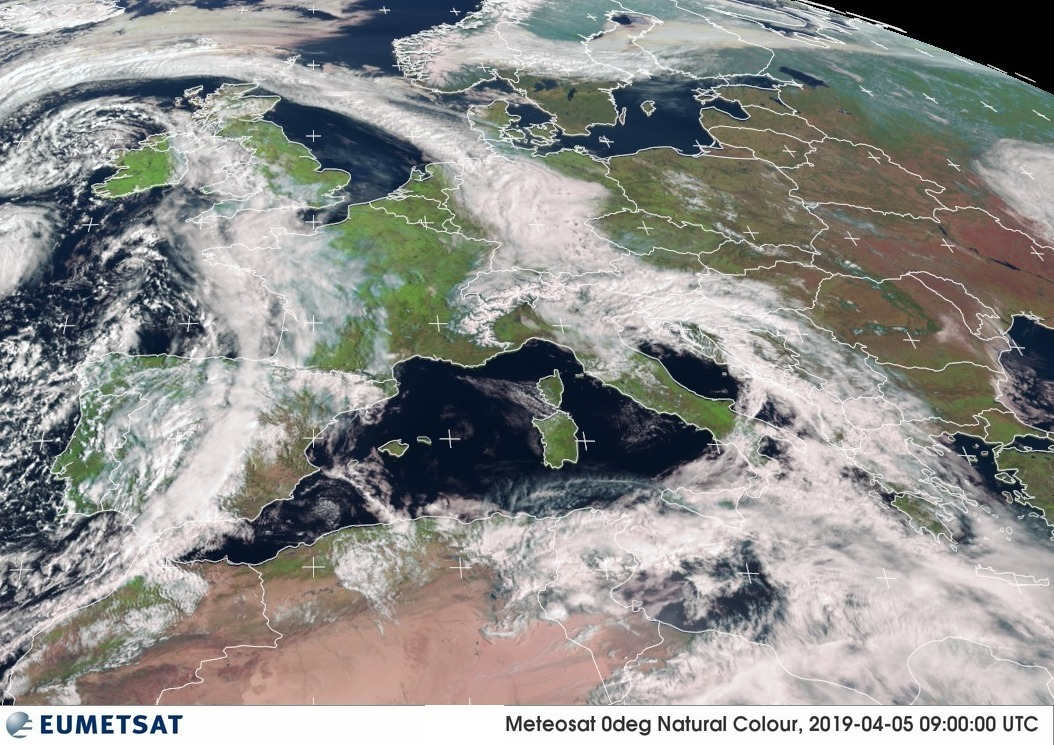
\includegraphics[width=6cm]{images/EUMETSAT/MET10_RGBNatColourEnhncd_CentralEurope_20190405090000}}
	\only<2>{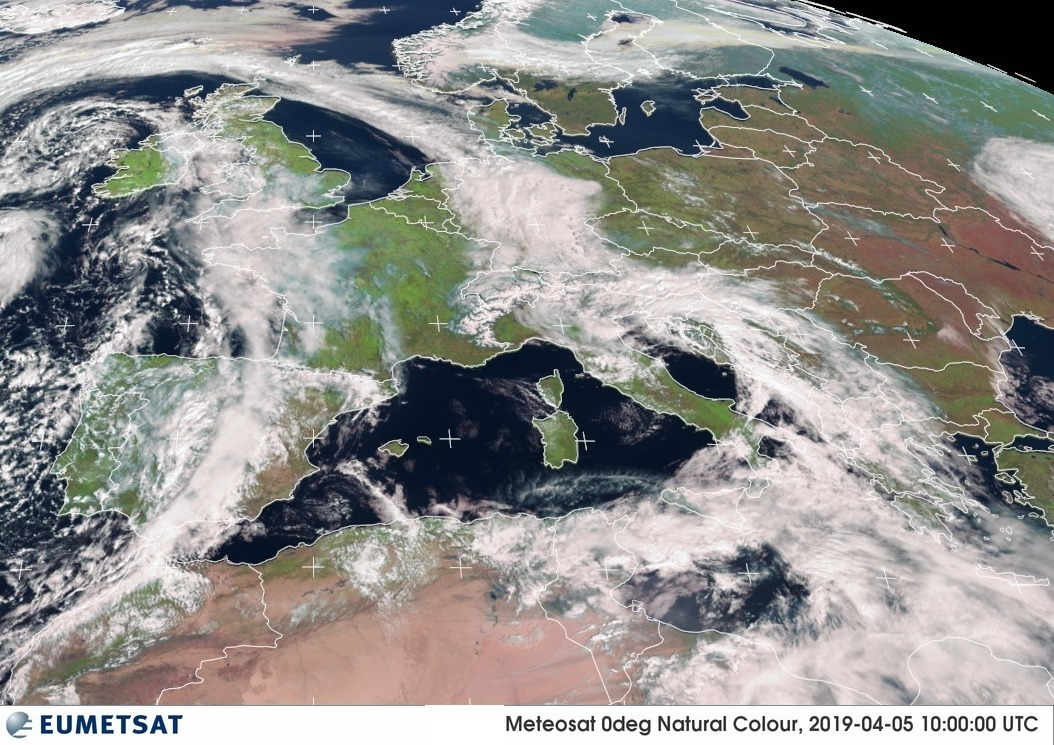
\includegraphics[width=6cm]{images/EUMETSAT/MET10_RGBNatColourEnhncd_CentralEurope_20190405100000}}
	\only<3>{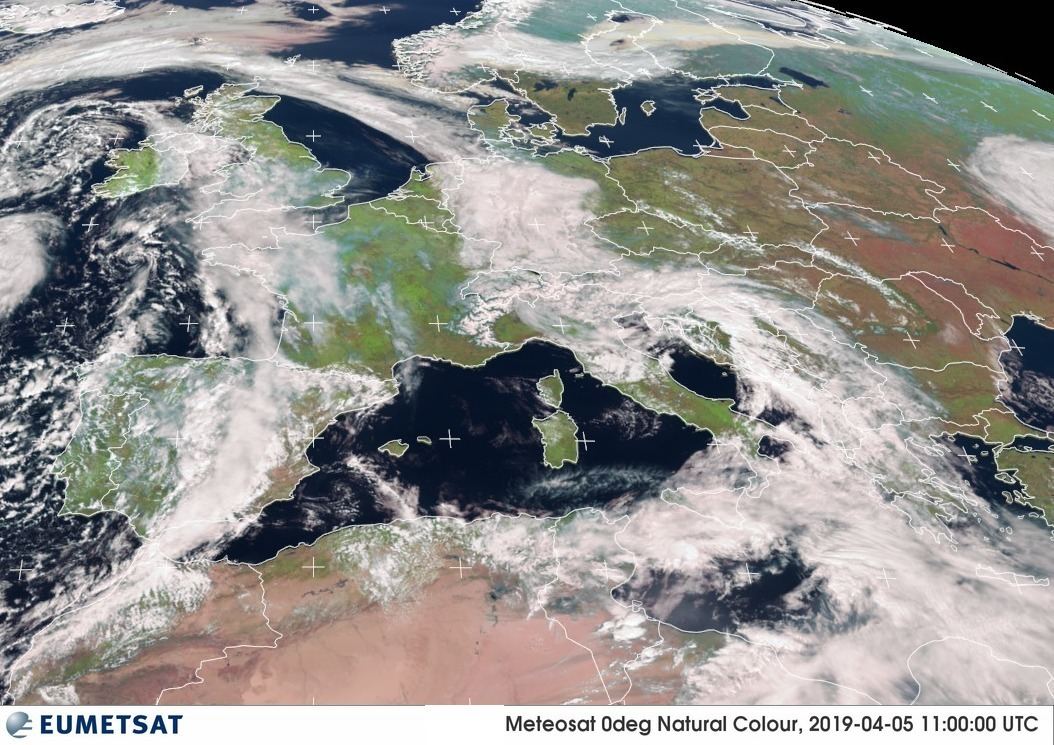
\includegraphics[width=6cm]{images/EUMETSAT/MET10_RGBNatColourEnhncd_CentralEurope_20190405110000}}
%	\only<4>{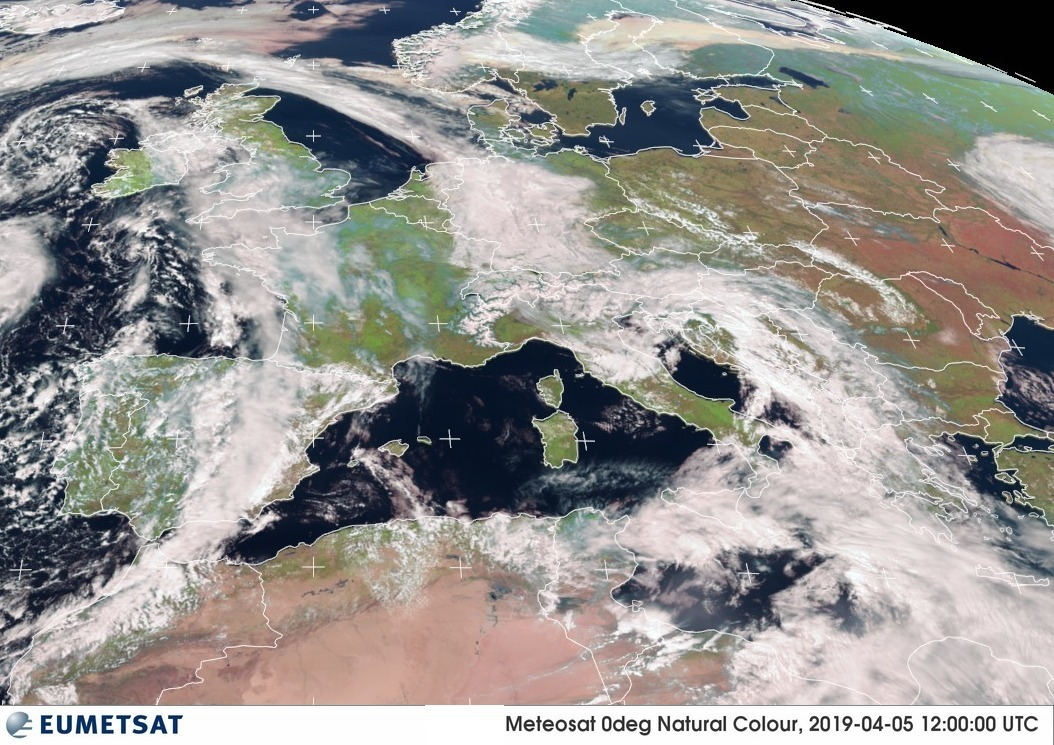
\includegraphics[width=6cm]{images/EUMETSAT/MET10_RGBNatColourEnhncd_CentralEurope_20190405120000}}
	
\end{columns}

\url{http://oiswww.eumetsat.org}
\hfill
\vfill
\scriptsize Icons from \url{https://www.flaticon.com}
\end{frame}
}

\begin{frame}
	\frametitle{Sun Synchronus Orbit}
	\begin{columns}
		\column{.66\textwidth}
		
%		Orbiting closer capture less area with higher spatial resolution.
%		The comparatively large earth Shadow forces these satellites on the sun synchornous orbit
		
		\textbf{Environmental Satellites} with 1km spatial resolution every day
		\begin{itemize}
			\item NASA's MODIS Aqua/Terra
			\item ESA's Sentinel 3
		\end{itemize}
		\vspace{2em}
		 
		\textbf{Multi-spectral satellites} with 10-60m spatial resolution 3-10 days
		\begin{itemize}
			\item NASA's Landsat Satellites (since 70s!)
			\item ESA's Sentinel 2
		\end{itemize}
		 
%		\begin{itemize}
%			\item 
%			\item 
%		\end{itemize}
		
		\column{.33\textwidth}
		
			\only<1-3>{
			\begin{tikzpicture}
			
			
			\draw [tumgraylight,dotted,domain=230:315] plot ({2*cos(\x)}, {2*sin(\x)});
			
			\visible<1>{
				\node[rotate=0, anchor=center](earth) at (0,0) {
\includegraphics[width=20mm]{images/icons/earth}};
				\node[anchor=center, rotate around={-20:(0,2)}](sat) at (0,-2) {
\includegraphics[width=5mm]{images/icons/sat2}};
				\draw[font=\tiny] (earth) -- node[midway,below,sloped]{800km} (sat);
			}
			\visible<2>{
				\node[rotate=0, anchor=center](earth) at (0,0) {
\includegraphics[width=20mm]{images/icons/earth}};
				\node[anchor=center, rotate around={0:(0,2)}](sat) at (0,-2) {
\includegraphics[width=5mm]{images/icons/sat2}};
				\draw[font=\tiny] (earth) -- node[midway,below,sloped]{800km} (sat);
			}
			\visible<3>{
				\node[rotate=0, anchor=center](earth) at (0,0) {
\includegraphics[width=20mm]{images/icons/earth}};
				\node[anchor=center, rotate around={20:(0,2)}](sat) at (0,-2) {
\includegraphics[width=5mm]{images/icons/sat2}};
				\draw[font=\tiny] (earth) -- node[midway,below,sloped]{800km} (sat);
			}
			\end{tikzpicture}
			}
%			
%			\only<4>{
%				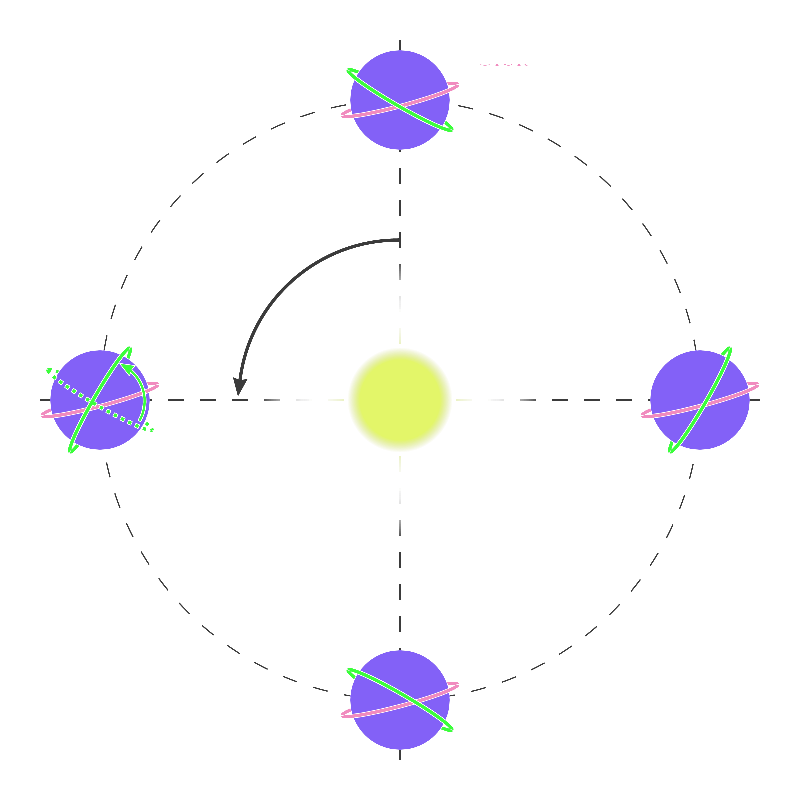
\includegraphics[width=5cm]{images/sso_white}
%			}
		
%			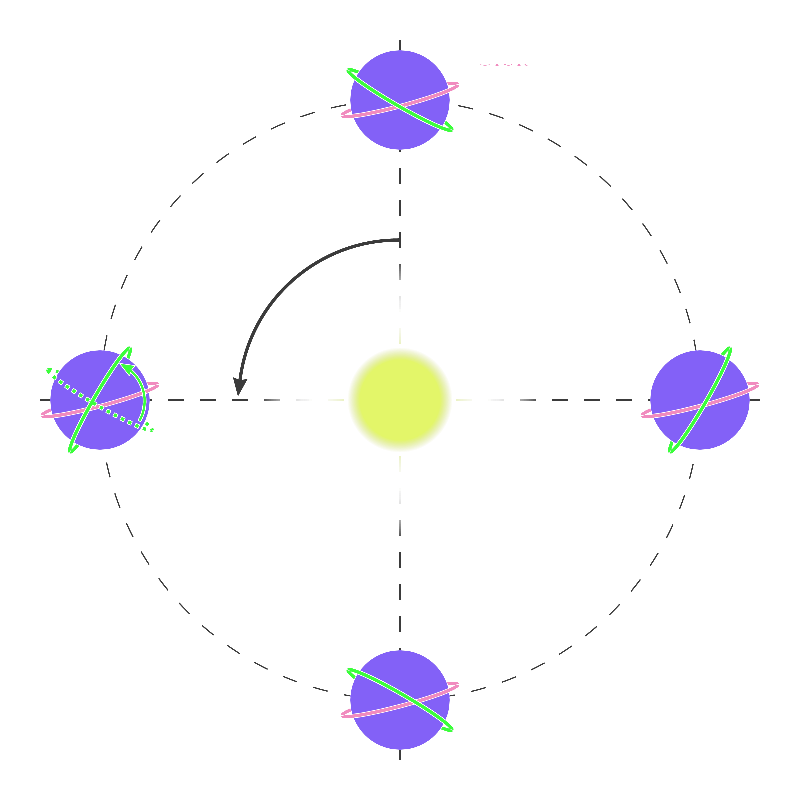
\includegraphics[width=.33\textwidth]{images/sso_white}
		
	\end{columns}
%	
%	image from \url{https://en.wikipedia.org/wiki/Sun-synchronous_orbit}
\end{frame}

\begin{frame}
	\frametitle{Global Environmental Satellites}
	
	\begin{columns}
		\column{.5\textwidth}
		
		Moderate Resolution Spectrometer
		\begin{itemize}
			\item images every day
			\item resolution $\approx 1km$
			\item $> 50$ spectral bands
		\end{itemize}
		
		\column{.5\textwidth}
		
		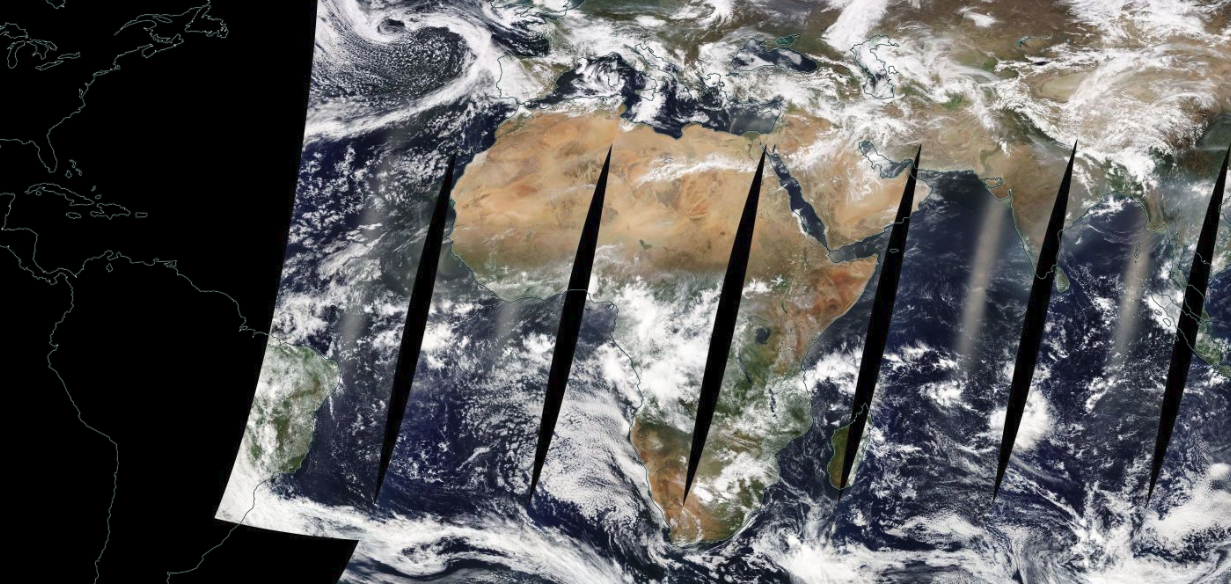
\includegraphics[width=\textwidth]{images/modis}
		
	\end{columns}
	
	\url{https://worldview.earthdata.nasa.gov/}
	
\end{frame}

\begin{frame}
	\frametitle{Multi Spectral Satellites -- Example Sentinel 2 or Landsat}
	
	\begin{columns}[t]
		
		\column{.5\textwidth}
		
		
		
		\textbf{USGS Landsat}
		\begin{itemize}
			\item spatial resolution 30m
			\item covers every point on Earth every 16 days
			\item 11 spectral bands
			\item since the 80s
		\end{itemize}
		
		\vspace{2em}
		
		\textbf{ESA Sentinel-2}
		\begin{itemize}
			\item spatial resolution 10m-60m
			\item covers every point on Earth every 2-5 days
			\item 13 spectral bands
			\item since 2016
		\end{itemize}
		
		\column{.5\textwidth}
		
		\includegraphics[width=\textwidth]{images/airbus_Sentinel-2_022415_945}
		
		©AIRBUS DEFENCE AND SPACE
	\end{columns}
	
	
	
\end{frame}

\begin{frame}
\frametitle{Multi Spectral Satellites -- Example Sentinel 2}

%\newcommand{\focusband}[1]{\color{tumorange} #1}

\begin{columns}
	\column{.33\textwidth}
%	
%	\color{tumgray}
	\only<1>{True Color}
	\only<2>{False Color}
	\only<3>{False Color Urban}
	\only<4>{Short-Wave Infra Red Bands}
	\only<5>{MoistureIndex}
	\only<6>{Vegetation Index (NDVI)}
	\only<7>{Water Index (NDWI)}
	
	\small
	\begin{equation*}
	\M{X} = \begin{pmatrix}
		\rho_{B1} \\ 
		\only<2,3,4,5,6,7>{\rho_{B2}} \only<1>{\color{tumorange}\rho_{B2}} \\
		\only<3,4,5,6>{\rho_{B3}} \only<1,2,7>{\color{tumorange}\rho_{B3}} \\
		\only<5,7>{\rho_{B4}} \only<1,2,3,4,6>{\color{tumorange}\rho_{B4}} \\
		\rho_{B5} \\
		\rho_{B6} \\
		\rho_{B7} \\
		\only<1,3,4,5>{\rho_{B8}} \only<2,6,7>{\color{tumorange}\rho_{B8}} \\
		\only<1,2,3,6,7>{\rho_{B8A}} \only<4,5>{\color{tumorange}\rho_{B8A}} \\
		\rho_{B9} \\
		\rho_{B10} \\
		\only<1,2,4,6,7>{\rho_{B11}} \only<3,5>{\color{tumorange}\rho_{B11}} \\
		\only<1,2,5,6,7>{\rho_{B12}} \only<3,4>{\color{tumorange}\rho_{B12}}
		\end{pmatrix} \xrightarrow{visualize} 
		\begin{pmatrix}
			\only<1>{\rho_{B4} \\ \rho_{B3} \\ \rho_{B2}}
			\only<2>{\rho_{B8} \\ \rho_{B4} \\ \rho_{B3}}
			\only<3>{\rho_{B12} \\ \rho_{B11} \\ \rho_{B4}}
			\only<4>{\rho_{B12} \\ \rho_{B8A} \\ \rho_{B4}}
			\only<5>{\frac{\rho_{B8A}-\rho_{B11}}{\rho_{B8A}+\rho_{B11}}}
			\only<6>{\frac{\rho_{B8}-\rho_{B4}}{\rho_{B8}+\rho_{B4}}}
			\only<7>{\frac{\rho_{B3}-\rho_{B8}}{\rho_{B3}+\rho_{B8}}}
		\end{pmatrix}
	\end{equation*}
	%\myvec{\rho_{\lambda_1} \\ \rho_{\lambda_2} \\ \dots \\ \rho_{\lambda_n}}
	
	\url{https://apps.sentinel-hub.com}
	
	\column{.66\textwidth}
	
	\only<1>{\includegraphics[width=\textwidth]{images/s2/RGB}}
	\only<2>{\includegraphics[width=\textwidth]{images/s2/FalseColor}}
	\only<3>{\includegraphics[width=\textwidth]{images/s2/FalseColor(urban)}}
	\only<4>{\includegraphics[width=\textwidth]{images/s2/SWIR}}
	\only<5>{\includegraphics[width=\textwidth]{images/s2/MoistureIndex}}
	\only<6>{\includegraphics[width=\textwidth]{images/s2/NDVI}}
	\only<7>{\includegraphics[width=\textwidth]{images/s2/NDWI}}
	
	
\end{columns}
%
%\vspace{2em}
%{\small
%\url{https://apps.sentinel-hub.com/eo-browser/?lat=51.75771\&lng=-1.25963\&zoom=15\&time=2019-04-20\&preset=7-NDWI\&datasource=Sentinel-2\%20L1C}
%}

\end{frame}


\begin{frame}

\vfill
\Huge\color{black}
\begin{center}
	\begin{columns}
		\column{\textwidth}
		\vspace{7em}
		
		\textbf{Takeaway:}
		\hfill 
		Each pixel has rich physical information
		%			\includegraphics[width=5cm]{images/dscovrepic/epic1}
		%\includegraphics[width=7cm]{images/fdl}
	\end{columns}
\end{center}

\vfill

\end{frame}


\begin{frame}
	\frametitle{Open Data Policy!}
	
%	So far all datasets are freely available to the public!
	
	\begin{columns}[t]
		\column{.5\textwidth}
		
		\Large
		\begin{itemize}
			\item This data is acquired globally
			\item at regular time intervals
			\item and is completely free to the public
		\end{itemize}
		
		\vspace{1em}
		\hspace{2em}\includegraphics[width=2cm]{images/usgs}
		\hspace{1em}
		\includegraphics[width=2cm]{images/modis_icon}
		
		\column{.5\textwidth}
		
		\includegraphics[width=6cm]{images/SentinelFleet}
		
	\end{columns}

	\vspace{1em}
	
	\small
	
	\url{https://wdc.dlr.de/sensors/modis/}
	
	\url{https://www.usgs.gov/land-resources/nli/landsat}
	
	\url{http://www.esa.int/spaceinimages/Images/2014/04/Sentinel_family}
	
	
\end{frame}

\begin{frame}
\frametitle{High (spatial) Resolution Satellites}
\begin{columns}
	\column{.33\textwidth}
	
	\begin{itemize}
		\item Highest spatial detail ($<1m$ spatial resolution).
		\item Images acquired on an acquisition schedule
	\end{itemize}
	
	\begin{equation*}
		\M{X} = \begin{pmatrix}
		\rho_\text{red} \\ 
		\rho_\text{green} \\
		\rho_\text{blue} \\
		\rho_\text{near-infrared}
		\end{pmatrix}
	\end{equation*}
	
	\vspace{1em}
	
	\includegraphics[width=1.5cm]{images/airbus}
	\hspace{1em}
	\includegraphics[width=1.5cm]{images/digitalglobe}
	
	\vspace{1em}
	\includegraphics[width=2cm]{images/planet}
	\includegraphics[width=1cm]{images/earthi}
	
	
	\column{.66\textwidth}
	
	\includegraphics[width=\textwidth]{images/wolfson_vhr.png}
	
\end{columns}
\end{frame}

\begin{frame}
	\frametitle{Computer Vision and High Resolution Data}
	
	\begin{columns}
		\column{.5\textwidth}
	
			\textbf{SpaceNet Challenge}
			\url{https://spacenetchallenge.github.io/}
			
			\vspace{2em}
			\textbf{Inria Aerial Labelling Dataset}
			\url{https://project.inria.fr/aerialimagelabeling/}
			
			\includegraphics[width=4cm]{images/spacenet}
			\includegraphics[width=6cm]{images/inriadataset}
		
		\column{.5\textwidth}
		
		\includegraphics[width=\textwidth]{images/inria_aerial_labels}
			
		
	\end{columns}
	
\end{frame}

\begin{frame}
	
	\vfill
	\Huge\color{black}
	\begin{center}
		\begin{columns}
			\column{\textwidth}
			\vspace{7em}
			
			\textbf{Takeaway:}
			\hfill 
			\only<1>{EO data has potential} \only<2>{only VHR has exposure in ML}
			%			\includegraphics[width=5cm]{images/dscovrepic/epic1}
			%\includegraphics[width=7cm]{images/fdl}
		\end{columns}
	\end{center}
	
	\vfill
	
\end{frame}

%
%{\setbeamercolor{background canvas}{bg=tumwhite}
%	\begin{frame}[plain]
%	
%	\vfill
%	\Huge\color{black}
%	\begin{center}
%		\begin{columns}
%			\column{\textwidth}
%			\vspace{7em}
%			
%			\textbf{Takeaway:}
%			\hfill 
%			\only<1>{EO data has huge potential} \only<2>{hardly any exposure in ML research}
%%			\includegraphics[width=5cm]{images/dscovrepic/epic1}
%			%\includegraphics[width=7cm]{images/fdl}
%		\end{columns}
%	\end{center}
%	
%	\vfill
%\end{frame}
%}


%
%\begin{frame}
%	\frametitle{Takeaway}
%	
%	\textbf{Earth Observation Data}
%	\begin{description}
%		\item[globally] available
%		\item[often free] of charge  
%	\end{description}
%
%	\textbf{text}
%	\item[complexity] of the data usually a limiting factor for broader adaptability
%
%	\textbf{Earth Observation and Maci}
%	
%\end{frame}

%
%\begin{frame}
%\frametitle{Image Super Resolution}
%
%\includegraphics[width=.8\textwidth]{images/superresolution}
%
%\url{https://mdl4eo.irstea.fr/2019/03/29/enhancement-of-sentinel-2-images-at-1-5m/}
%
%\end{frame}
%
%\begin{frame}
%	\frametitle{Diverse Data}
%\end{frame}

%
%\begin{frame}
%	\newcommand{\bblock}[6]{
	\draw[#1] (axis cs: #2,#4) rectangle node[text=white]{#6} (axis cs: #3,#5);
}

\newcommand{\event}[2]{
	\draw[draw=tumblue] (axis cs: #1,0) -- (axis cs: #1,8) node[above,font=\small]{#2};
}

\begin{tikzpicture}
\tikzstyle{project}=[fill=tumblue, draw=none, font=\tiny]
\tikzstyle{phase}=[fill=tumgray, draw=none, font=\small]
\tikzstyle{futureproject}=[fill=tumblue, draw=none, font=\tiny, fill opacity=0.2]
\tikzstyle{conference}=[fill=tumorange, draw=none, very thick, font=\tiny]

\begin{axis}[
	date coordinates in=x,
	xticklabel=\year,
	xtick={2019-01-01,2020-01-01,2021-01-01},
	width=\textwidth,
	height=6cm,
	ymax=10,
	ymin=-5,
	xmin=2018-05-01,
	xmax=2021-09-01,
	hide y axis,
	axis line style={draw=none}]
	
	\event{2018-06-01}{start}
	\bblock{project}{2018-06-25}{2018-08-17}{1}{2}{FDL}
	\bblock{project}{2018-10-01}{2019-2-15}{2}{3}{IRISA Obelix}
%	\block{conference}{2018-12-01}{2018-12-06}{4}{5}{NeurIPS}
%	\block{conference}{2018-11-12}{2018-11-16}{5}{6}{$\Phi$-week}
%	\block{conference}{2019-01-27}{2019-02-01}{5}{6}{AAAI}
	\event{2019-02-10}{this exposé}
	\bblock{project}{2019-3-01}{2019-10-01}{3}{4}{crop type mapping}
	%\block{project}{2019-8-01}{2019-10-15}{2}{3}{ESA}
	\bblock{futureproject}{2019-10-01}{2020-06-01}{4}{5}{biomass and crop yield}
	\bblock{futureproject}{2020-06-01}{2020-12-31}{5}{6}{nowcasting of atmospheric effects}
	\bblock{futureproject}{2021-01-01}{2021-06-01}{6}{7}{writing}
	\event{2021-06-01}{defense}
	
	\draw[left color=tumbluelight, right color=tumbluedark, draw=none, fill opacity=0.2] (axis cs: 2018-06-01,-2) rectangle node[left=10em, font=\small]{supervised} node[text=white, font=\small]{semi-supervised} node[right=9em, text=white, font=\small]{unsupervised} (axis cs: 2021-06-01,-1);
	
	\bblock{phase}{2018-06-01}{2018-11-31}{-4}{-3}{warm-up}
	\bblock{phase}{2019-02-01}{2020-11-31}{-4}{-3}{research}
	\bblock{phase}{2021-02-01}{2021-06-01}{-4}{-3}{wrap-up}
	
%\addplot [red] expression {1/(1+exp(-x))};  % <-- fails if uncommented
\end{axis}
\end{tikzpicture}

%\end{frame}

